\documentclass[5p,times,twocolumn]{elsarticle}

% ============================================================
% PACKAGES
% ============================================================
\usepackage[T1]{fontenc}
\usepackage[utf8]{inputenc}
\usepackage{amsmath,amssymb}
\usepackage{graphicx}
\usepackage{booktabs}
\usepackage{siunitx}
\usepackage{xcolor}
\usepackage[protrusion=true,expansion=true]{microtype}
\usepackage[hidelinks]{hyperref}
\usepackage{multirow}
\usepackage{array}
\usepackage{tabularx}

\sisetup{separate-uncertainty=true}
\graphicspath{{figures/}}

\newcolumntype{C}[1]{>{\centering\arraybackslash}p{#1}}

\journal{Acta Materialia}

% ============================================================
% FRONT MATTER
% ============================================================
\begin{document}

\begin{frontmatter}

\title{Revisiting Hall--Petch strengthening in FCC high-entropy alloys: best practices for building and auditing machine-learning strength models}

\author[mse]{Mrinalini~Mulukutla\corref{cor1}}
\ead{mrinalini.mulukutla@tamu.edu}
\author[mse]{Shakti~Prasad~Padhy}
\author[mse]{Wenle~Xu}
\author[mse]{Bibhu~Prasad~Sahu}
\author[mse]{Ibrahim~Karaman}
\author[mse]{Raymundo~Arr\'{o}yave}
\cortext[cor1]{Corresponding author.}

\affiliation[mse]{organization={Department of Materials Science and Engineering, Texas A\&M University},
  city={College Station},
  state={TX},
  postcode={77843},
  country={USA}}

\begin{abstract}
Machine-learning (ML) property models can mislead, or actively harm, alloy design when physics, descriptors, validation strategy, and deployment limits are not handled with care. We present a best-practices framework that instead uses ML to construct \emph{and} audit physics-informed models, and we demonstrate it end-to-end on the yield strength (YS) and Vickers hardness (HV) of 94 FCC high-entropy alloys in the Al--Co--Cr--Cu--Fe--Mn--Ni--V system (YS 152--544~\si{MPa}, grain size 15--212~\si{\micro\meter}). The framework is a controlled ascent in model flexibility---classical Hall--Petch, composition--processing linear models, physics-informed descriptors, a non-linear ML panel (ARMOTE-CV), and symbolic regression (PySR, SISSO)---with every tier evaluated on a shared feature ladder under 5-fold, leave-one-out (LOO), leave-one-batch-out (LOBO), and external validation. Each tier gains predictive capability and incurs a specific, named risk: faithfully implemented solid-solution-strengthening models overpredict by factors of 2--28 and become redundant once composition is present (partial $r < 0.10$); rule-of-mixtures means are inert while a grain-size-heterogeneity term ($\text{SD}_\text{grain}\cdot d^{-1/2}$) governs strengthening; LOO flatters models that LOBO exposes (XGBoost $0.729 \to 0.574$); and the best-BIC closed-form law hides a singularity that fails on independent data (external RMSE $421 \to 163$~\si{MPa} for a bounded variant). For YS, symbolic regression gives the most accurate interpretable model (PySR, LOO $R^2 = 0.77$, LOBO $R^2 = 0.67$), and three independent engines---PySR, SISSO, and a Bayesian composition-dependent Hall--Petch model---converge on the same $\text{SD}_\text{grain}\cdot d^{-1/2}$ form, which we read as genuine physics rather than a fitting artifact. For HV the same protocol correctly flags that composition overfits (all composition models LOO $R^2 \leq 0.14$) and that hardness is grain-geometry-dominated. The particular coefficients are alloy-specific; the protocol---physics-anchored feature ladders, descriptor-redundancy audits, variance-over-means descriptors, cluster-out validation, and singularity audits---is material-class-agnostic and is offered as a reusable workflow for sparse, clustered materials data.
\end{abstract}

\begin{keyword}
High-entropy alloys \sep Hall--Petch \sep Machine learning \sep Symbolic regression \sep Cross-validation \sep Hardness
\end{keyword}

\end{frontmatter}

% ============================================================
% 1. INTRODUCTION
% ============================================================
\section{Introduction}
\label{sec:intro}

Multi-principal element alloys (MPEAs), including high-entropy alloys (HEAs), have emerged over the past two decades as a class of structural materials whose mechanical properties arise from cooperative interactions among multiple alloying elements in concentrated solid solutions~\cite{Cantor2004,Yeh2004,George2019}.
Unlike conventional alloys built around a single principal element with dilute additions, MPEAs occupy vast compositional regions in which yield strength, ductility, and fracture resistance are jointly governed by lattice distortion, local chemical ordering, and microstructural parameters such as grain size~\cite{Miracle2017}.
With eight elements, allowing non-equiatomic variants expands the search space to a continuous high-dimensional simplex containing $\gtrsim 10^9$ distinct compositions at 1~at.\% resolution, with processing variables (cold work, recrystallization temperature, hold time) adding further dimensions~\cite{Senkov2018}.
Practical alloy development under these constraints increasingly relies on machine-learning (ML) surrogates trained on modest experimental datasets, and closed-loop ML-driven campaigns have begun to deliver on that promise: active learning discovered high-entropy Invar alloys after synthesizing only 17 of millions of candidates~\cite{Rao2022}, and risk-aware batch Bayesian optimization produced the dataset analyzed in this work~\cite{Mulukutla2024BIRDSHOT,Mulukutla2026BRAVE}.
This reliance is exactly where the risk lies.
Random-split cross-validation systematically overestimates model performance for discovery tasks, because deployment requires extrapolation to new regions of composition space while random splits test only interpolation~\cite{Meredig2018}; an ML property model that scores well under a permissive validation protocol can therefore silently fail when deployed on new compositions, new processing routes, or new laboratories.
The premise of this paper is that ML property prediction becomes misleading---or actively detrimental to a design campaign---when four things are mishandled: the physics encoded in the features, the redundancy of hand-built descriptors, the validation strategy, and the deployment limits of the fitted model.
Handled carefully, the same ML machinery can instead both \emph{construct} predictive models and \emph{audit} physics-informed ones. We develop and demonstrate that dual use here.

Grain size is the natural backbone for any strength model of polycrystalline alloys.
The Hall--Petch (HP) relationship, $\sigma_y = \sigma_0 + k_\text{HP}\,d^{-1/2}$, has served as the foundational empirical description of grain-size strengthening for over seven decades~\cite{Hall1951,Petch1953}, with the $d^{-1/2}$ scaling derivable from both dislocation pile-up and geometrically-necessary-dislocation arguments~\cite{Cordero2016}.
Reported HEA slopes can substantially exceed pure-FCC values---e.g., $k_\text{HP} \approx 494$~MPa$\cdot\mu$m$^{1/2}$ for CoCrFeMnNi at room temperature~\cite{Otto2013} versus ${\approx}110$--160~MPa$\cdot\mu$m$^{1/2}$ for pure Cu and Ni~\cite{Cordero2016}---although CoCrNi shows a more moderate slope accompanied by an unusually high friction stress~\cite{Yoshida2017}.
Alternative scaling laws ($d^{-1}$ from source-limited arguments~\cite{Dunstan2014}, $d^{-1/3}$~\cite{Baldwin1958}, $\ln(d)/d$~\cite{Li2016HP}) coexist in the literature, often supported by curve-fit goodness-of-fit but rarely discriminated by information-theoretic comparison, and their applicability to MPEAs remains largely untested.
The model FCC systems illustrate why the decomposition matters: CoCrFeMnNi combines a moderate friction stress (${\sim}125$~\si{MPa}) with a steep slope~\cite{Otto2013}, whereas CoCrNi shows a more moderate slope ($k_\text{HP} \approx 265$~MPa$\cdot\mu$m$^{1/2}$) alongside an unusually high friction stress ($\sigma_0 \approx 218$~\si{MPa}, versus ${\sim}14$~\si{MPa} for pure Ni)~\cite{Yoshida2017}.
These observations raise the question---answered quantitatively at Tier~3 of this work---of whether elevated HEA intercepts and slopes reflect composition-dependent grain-boundary strengthening or a composition-dependent friction stress absorbed into the slope through fitting.
Systematic friction-stress extractions across CoCrFeMnNi subsets show the intercept varying strongly with elemental combination~\cite{Yoshida2019acta}, while recent measurements show the slope itself responding to boundary chemistry: Mo grain-boundary segregation raises $k_\text{HP}$ to 1100~MPa$\cdot\mu$m$^{1/2}$ in an FCC HEA, among the largest values reported for any FCC alloy~\cite{LiKHP2024}.
Disentangling the two channels therefore requires fitting them jointly, not reading either off a global regression.

Above the grain-size backbone sits composition. The friction stress $\sigma_0$ depends on chemistry through solid-solution strengthening (SSS): the Varvenne--Leyson--Curtin (VLC) framework computes SSS from atomic-volume misfit variance~\cite{Varvenne2016,Varvenne2017}, while the Labusch and Toda-Caraballo approaches use different combinations of size and modulus misfit~\cite{Labusch1970,TodaCaraballo2015}.
These models can be evaluated with Vegard's-law-interpolated inputs or with first-principles volumes~\cite{Yin2020,Moitzi2022}.
Heuristic descriptor sets developed for HEA phase prediction---atomic-size mismatch $\delta$, valence electron concentration VEC, mixing enthalpy and entropy, the stability parameter $\Omega$, electronegativity mismatch---further extend the candidate feature space~\cite{Zhang2008,Yang2012,Guo2011,Troparevsky2015,Ye2015geometric,Ye2015phi}, and Wen et al.\ showed that hybrid physics--ML formulations can outperform purely physics-based SSS baselines~\cite{Wen2021SSS}.
ML has been applied widely to HEA property prediction~\cite{Huang2019,Islam2022,Wen2019,Rickman2019,Khatamsaz2023,LiuPei2023}, but most mechanical-property studies share three limitations~\cite{Hart2021}: (i) composition-only descriptors without explicit grain-size effects---an omission that recent studies themselves flag as their key limitation, (ii) a narrow model panel without systematic comparison, and (iii) validation by random-split cross-validation alone, without cluster-out or external tests, despite community best-practice guidance to the contrary~\cite{WangAYT2020}.
Each limitation maps onto a concrete failure mode that we measure in this work: descriptor redundancy, validation optimism, and deployment failure of closed-form models.

We address these gaps with a framework that reads as a single controlled ascent in model flexibility, where each tier buys predictive capability and incurs a specific, named risk that the framework then manages:
(1)~the universal backbone---classical Hall--Petch on grain size alone;
(2)~composition and processing in interpretable linear models (the M-model hierarchy), revealing where the signal lives ($\sigma_0$ versus $k_\text{HP}$);
(3)~domain physics descriptors (SSS, Wen-type, PCA), testing whether hand-built physics helps and exposing the redundancy failure mode;
(4)~non-linear flexibility (the ARMOTE-CV panel), capturing interactions automatically and exposing the validation failure mode; and
(5)~symbolic regression (PySR, SISSO), recovering interpretable closed-form laws and exposing the deployment failure mode.
A validation floor runs under all five tiers---5-fold, leave-one-out (LOO), leave-one-batch-out (LOBO), and external validation, plus a singularity audit of every closed form---so that each step answers the question a practitioner in any material system must ask: did we gain, and at what risk?
Figure~\ref{fig:framework} summarizes the framework.

A second, equally deliberate design choice is that we carry two properties---yield strength (YS) and Vickers hardness (HV)---through the identical ladder, side by side.
The two properties give opposite answers: composition is signal for YS (it shifts $\sigma_0$; our M3 model reaches LOBO $R^2 = 0.625$) but noise for HV (every composition model overfits, LOO $R^2 \leq 0.14$), where strength is instead governed by grain geometry through a grain-size-heterogeneity term $\text{SD}_\text{grain}\cdot d^{-1/2}$.
A single ``universal'' model would mislead for at least one property; the fact that the same protocol exposes the contrast is itself the argument that property-specific modeling matters.

The main contributions are:
\begin{enumerate}
  \item A best-practices framework---feature ladder, descriptor-redundancy audit, three-protocol cross-validation, external validation, and singularity audit---in which ML both constructs and audits physics-informed strength models. Four measured failure modes (physics, descriptors, validation, deployment) are each paired with a guardrail.
  \item A composition-dependent Hall--Petch decomposition showing that composition enters through $\sigma_0$ and not $k_\text{HP}$ ($R^2 = 0.006$ for per-alloy $k_\text{HP}$ regression), with V the dominant strengthener ($\alpha_V = +291$~\si{MPa}), and a global $k_\text{HP} = 766$~MPa$\cdot\mu$m$^{1/2}$.
  \item Grain-size standard deviation ($\text{SD}_\text{grain}$) as a first-class predictor: the Bayesian model M15 ($= $ M3 $+$ $\text{SD}_\text{grain}\cdot d^{-1/2}$) ranks first by PSIS-LOO stacking weight with LOO $= $ LOBO $= 0.694$, and the same structural form is independently rediscovered by both symbolic-regression engines for both properties.
  \item An equal-footing comparison of linear, non-linear, and symbolic models on identical feature ladders and identical splits, showing that the Wen-type descriptors---not the model class---carry the YS signal, and that the best linear model matches or beats the non-linear panel cross-cluster.
  \item A deployment-aware model-selection table (LOO, LOBO, BIC, external RMSE, singularity safety) in place of a single leaderboard, with an explicit demonstration that the best-BIC equation is unsafe to deploy (external RMSE 421~\si{MPa}) while a bounded variant is safe (163~\si{MPa}).
\end{enumerate}

The remainder of this paper is organized as follows.
Section~\ref{sec:data} summarizes the dataset; detailed exploratory analysis is provided as Supplementary Information (SI).
Section~\ref{sec:methods} describes the four method families and the validation protocol.
Section~\ref{sec:results} presents results tier by tier, treating YS and HV in parallel throughout.
Section~\ref{sec:discussion} distills which method suits which property and why, states the transferable protocol, and discusses limitations. Section~\ref{sec:conclusions} concludes.

\begin{figure*}[t]
  \centering
  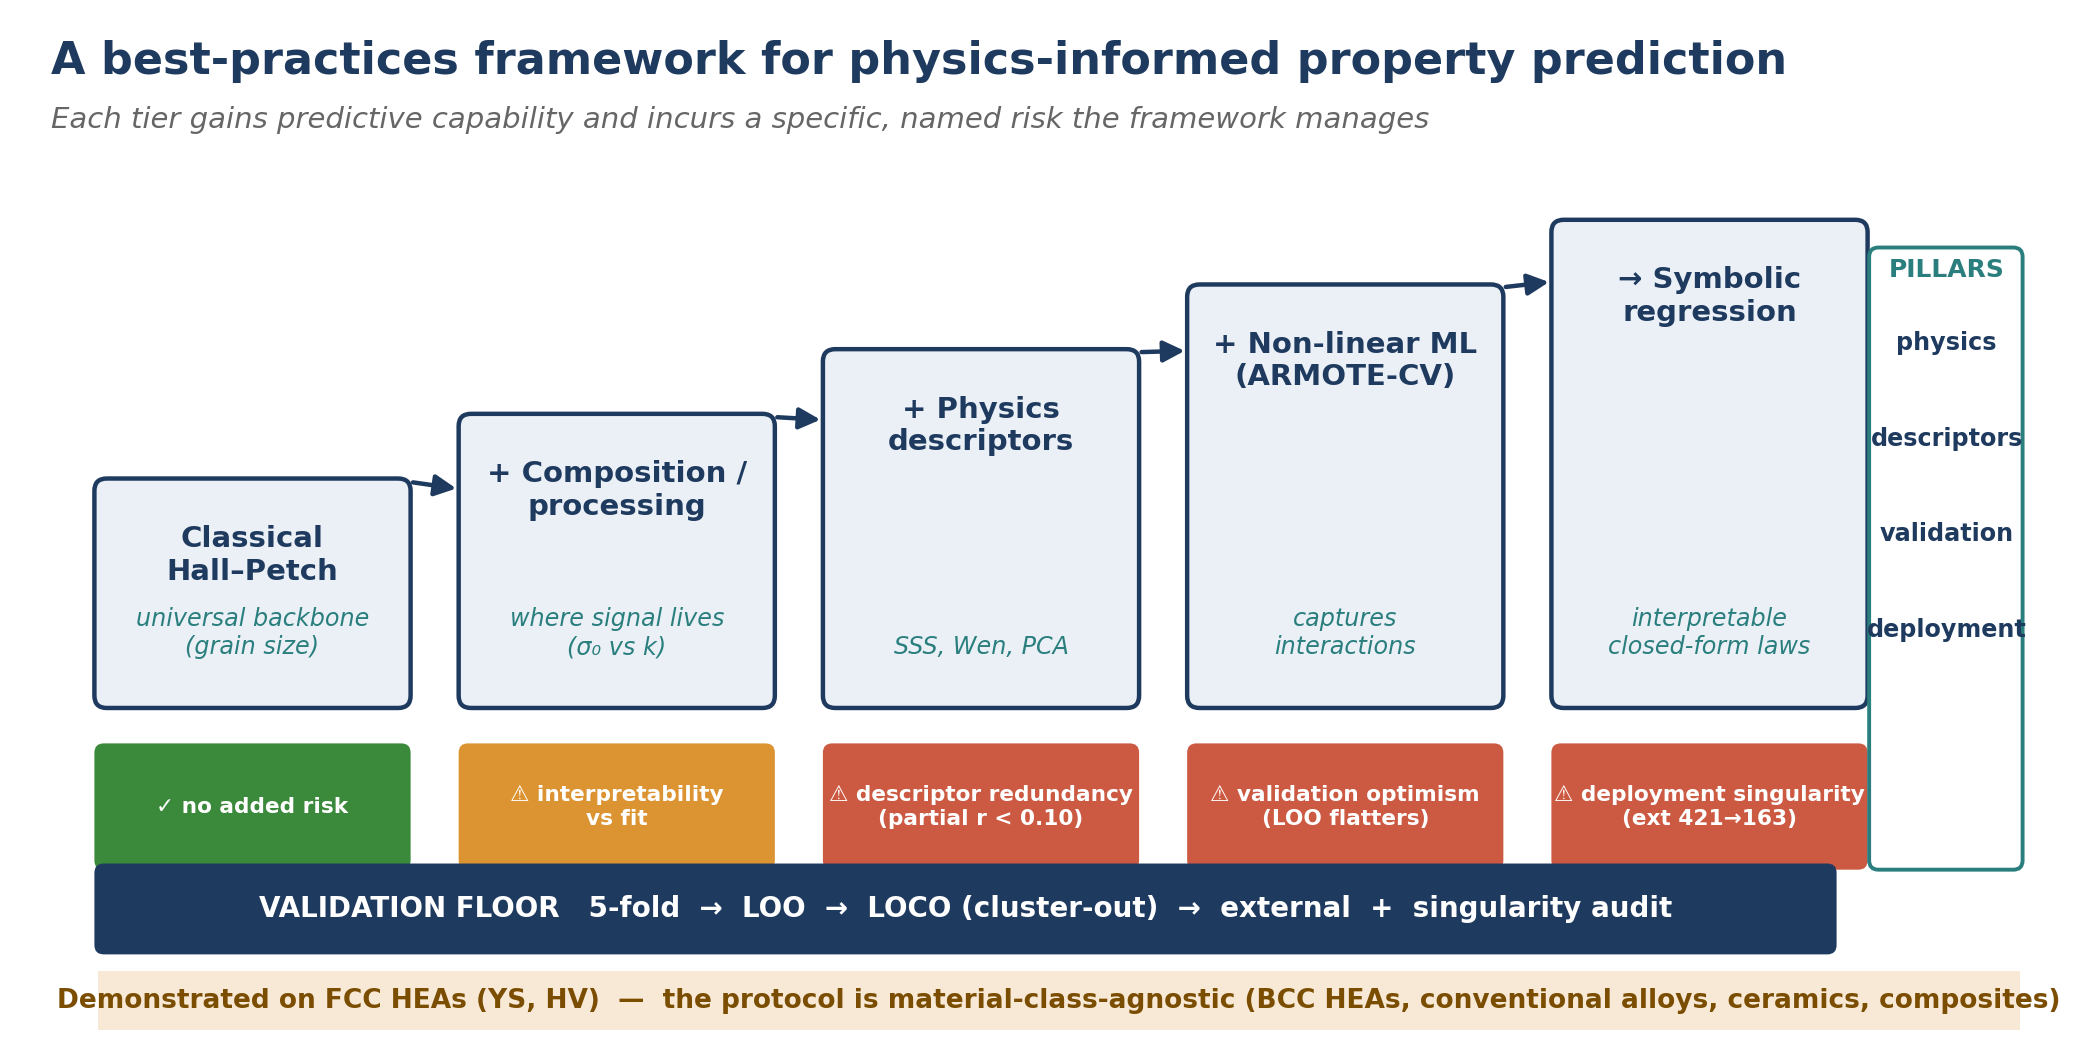
\includegraphics[width=\textwidth]{fig00_framework_overview.png}
  \caption{Framework overview. Five tiers of increasing model flexibility (classical Hall--Petch $\to$ composition/processing linear models $\to$ physics descriptors $\to$ non-linear ML $\to$ symbolic regression), each annotated with the capability gained and the risk incurred. A validation floor (5-fold $\to$ LOO $\to$ LOBO $\to$ external $+$ singularity audit) runs under all tiers; the right panel lists the four pillars (physics, descriptors, validation, deployment) and their guardrails. Demonstrated on FCC HEAs (YS, HV); the protocol is material-class-agnostic.}
  \label{fig:framework}
\end{figure*}

% ============================================================
% 2. DATA
% ============================================================
\section{Data}
\label{sec:data}

The dataset comprises 94 FCC HEAs in the Al--Co--Cr--Cu--Fe--Mn--Ni--V system (93 with yield-strength measurements, all 94 with Vickers hardness), produced in two Bayesian-optimization (BO) campaigns at Texas A\&M University under the BIRDSHOT initiative within the ARL HTMDEC program~\cite{Mulukutla2024BIRDSHOT,Hastings2025FCC}.
The first contributing campaign (batches BBA, BBB, BBC; 34 alloys) varied only chemistry over the eight-element space under a single FCC phase-stability constraint, with thermomechanical processing held fixed (60\% cold reduction, recrystallization at 950~\si{\degreeCelsius} for 0.5~h, water quench).
This campaign is documented in full in a companion paper~\cite{Mulukutla2026BRAVE}: a risk-aware Bayesian optimization in which a learned feasibility classifier, integrated into the multi-objective acquisition function, penalized candidates likely to fail at the phase-stability boundary; 48 alloys were synthesized over the three closed-loop iterations from ${\sim}27\,000$ CALPHAD-screened candidates, and the 34 with complete tensile, hardness, and EBSD characterization enter the present dataset.
The second campaign (batches CBA, CBB, CBC; 59 alloys) is a microstructure-aware BO over a six-element Co--Cr--Fe--Mn--Ni--V subspace ($c_\text{Al} = c_\text{Cu} = 0$) in which cold work (40--60\%), recrystallization temperature (675--1250~\si{\degreeCelsius}), and hold time (0.5--8~h) are design variables alongside composition, supplying wide within-composition grain-size variation.
All ingots were vacuum-arc-melted from $>99.9$~wt.\% precursors, homogenized, cold-rolled, recrystallized, and water-quenched; realized compositions were verified by EDS with mean ingot-level deviations of 0.4--0.6~at.\% from target~\cite{Mulukutla2024BIRDSHOT}.

Grain sizes, measured by EBSD on surfaces normal to the rolling direction, range from 15 to 212~\si{\micro\meter}.
For each alloy we also record the within-alloy standard deviation of the grain-size distribution, $\text{SD}_\text{grain}$, extracted from the same EBSD equivalent-circle-diameter distributions; this quantity enters the analysis as a first-class predictor rather than a quality-control statistic.
Yield strengths from quasistatic uniaxial tensile tests (0.2\% offset, $5\times10^{-4}$~s$^{-1}$) range from 152 to 544~\si{MPa}; Vickers hardness ranges from 58 to 228.
Table~\ref{tab:dataset} summarizes composition, processing, and property statistics.
The six BO batches represent distinct design iterations with overlapping but non-identical composition subspaces, providing the natural cluster structure for the LOBO protocol of Section~\ref{sec:validation}.
Because both campaigns are BO-driven, the alloys are not a random sample of the composition simplex; predictive $R^2$ values reported here should not be extrapolated to general-population alloys, and LOBO folds differ in difficulty (mean pairwise composition-hull overlap 0.21 in the leading PCA plane).
Full exploratory data analysis, property distributions, batch-coverage maps, and pre-modeling diagnostics---including the $\sigma_0$/$k_\text{HP}$ identifiability analysis and the noise-limited $R^2$ ceiling of ${\approx}0.97$ implied by replicate tensile tests---are given in SI Sections~S1--S2.

\begin{table}[t]
\centering
\caption{Dataset summary: composition, processing, and mechanical-property statistics.}
\label{tab:dataset}
\small
\begin{tabular}{lccc}
\toprule
Quantity & Min & Max & Mean $\pm$ SD \\
\midrule
\multicolumn{4}{l}{\textit{Composition (at.\%)}} \\
Al & 0 & 4 & $1.1 \pm 1.8$ \\
Co & 0 & 52 & $19.7 \pm 15.1$ \\
Cr & 0 & 20 & $8.1 \pm 5.1$ \\
Cu & 0 & 24 & $1.9 \pm 4.6$ \\
Fe & 0 & 32 & $11.1 \pm 7.8$ \\
Mn & 0 & 24 & $9.3 \pm 4.9$ \\
Ni & 16 & 72 & $40.6 \pm 13.0$ \\
V  & 0 & 24 & $8.3 \pm 6.3$ \\
\midrule
\multicolumn{4}{l}{\textit{Processing}} \\
Cold work (\%)              & 40 & 60   & $54.5 \pm 7.3$ \\
$T_\text{rx}$ ($^\circ$C)   & 675 & 1250 & $988 \pm 133$ \\
Hold time (h)               & 0.5 & 8    & $2.0 \pm 2.3$ \\
\midrule
\multicolumn{4}{l}{\textit{Mechanical properties \& grain size}} \\
YS (MPa)        & 152 & 544 & $269 \pm 82$ \\
HV              & 58  & 228 & $133 \pm 33$ \\
$d$ ($\mu$m)    & 15  & 212 & $58 \pm 43$ \\
\bottomrule
\end{tabular}
\end{table}

% ============================================================
% 3. METHODS
% ============================================================
\section{Methods}
\label{sec:methods}

The methods fall into four buckets that mirror the tiers of Fig.~\ref{fig:framework}: linear and physics-informed models (Section~\ref{sec:methods_linear}), the non-linear ML panel (Section~\ref{sec:methods_nonlinear}), symbolic regression (Section~\ref{sec:methods_sr}), and the validation protocol that runs under all of them (Section~\ref{sec:validation}).
All model families draw on a single shared feature ladder (Table~\ref{tab:ladder}) assembled into one prepared input file, so that every comparison in Section~\ref{sec:results} is made on identical inputs and identical splits.

\begin{table}[t]
\centering
\caption{The cumulative S1--S5 feature ladder. Each tier adds features to the previous one; S5 replaces hand-engineered interactions with symbolic-regression discovery. Rule-of-mixtures means ($\bar{\mu}$, $\delta_\mu$, $\bar{T}_m$, $\bar{a}$) are excluded from S4 because they never survive symbolic model selection and their removal barely moves the fit (Section~\ref{sec:tier4}).}
\label{tab:ladder}
\footnotesize
\setlength{\tabcolsep}{4pt}
\begin{tabular}{@{}lcp{4.6cm}@{}}
\toprule
Tier & \# feat & Content \\
\midrule
S1 grain & 2 & $d^{-1/2}$, $\text{SD}_\text{grain}$ \\
S2 $+$Wen & 8 & S1 $+$ curated Wen descriptors: VEC, $\Delta H_\text{mix}$, $\Delta S_\text{mix}$, $\Omega$, $\Delta\chi$, $\delta$ \\
S3 $+$proc & 11 & S2 $+$ cold work, $T_\text{rx}$, hold time \\
S4 $+$comp/SSS & 24 & S3 $+$ 8 element fractions $+$ $\sigma_\text{VLC}$, $\sigma_\text{Labusch}$, $\sigma_\text{TC}$, $\Phi_\text{VLC}$, $\varepsilon_L$ \\
S5 symbolic & --- & symbolic regression discovers the interactions (PySR, SISSO) \\
\bottomrule
\end{tabular}
\end{table}

\subsection{Linear and physics-informed models}
\label{sec:methods_linear}

\emph{(a) Classical and alternative grain-size scaling laws.}
Using grain size and $\text{SD}_\text{grain}$ only, we compare nine scaling laws of the form $\sigma_y = \sigma_0 + \sum_j k_j f_j(d)$ with $f(d) \in \{d^{-1/2}, d^{-1}, d^{-1/3}, d^{-2/3}, \ln(d)/d, \ln d, d^{-1/2}{+}d^{-1}, d^{-1}{+}d^{-2}, d^{-n_\text{opt}}\}$~\cite{Hall1951,Petch1953,Dunstan2014,Baldwin1958,Li2016HP}.
Frequentist comparison uses AIC, its small-sample correction AICc, and BIC~\cite{Akaike1974,Schwarz1978}, interpreted through the Burnham--Anderson and Kass--Raftery thresholds~\cite{BurnhamAnderson2002,KassRaftery1995}; Bayesian comparison uses MCMC-sampled posteriors (PyMC) scored by Pareto-smoothed importance-sampling LOO (PSIS-LOO)~\cite{Vehtari2017} with stacking weights~\cite{Yao2018}.
The same nine laws are fit to HV.
Within-replicate fits on the nine multi-replicate composition groups isolate the grain-size dependence from composition scatter (SI Section~S4).

\emph{(b) Composition--processing Hall--Petch hierarchy (M-models).}
We compare models of the form $\sigma_y = \sigma_0(\text{comp}) + k(\text{comp})\,d^{-1/2}$ spanning composition-dependent $\sigma_0$ only (M1: V; M3: all seven non-Ni fractions), composition-dependent $k$ only (M4, M6), both (M7--M10), and physics-descriptor variants (M11, M12).
Two $\text{SD}_\text{grain}$-augmented members extend the hierarchy: M13 adds $\text{SD}_\text{grain}$ to $\sigma_0$, and M15 $=$ M3 $+$ $\text{SD}_\text{grain}$ $+$ $\text{SD}_\text{grain}\cdot d^{-1/2}$.
The hierarchy is ranked by Bayesian PSIS-LOO stacking weight in addition to LOO/LOBO $R^2$ and BIC, and the identical hierarchy is run on HV with $H_0(\text{comp})$ in place of $\sigma_0(\text{comp})$.
A two-stage analysis (subtracting the fitted $\sigma_0(\text{comp})$ and regressing the implied per-alloy $k_\text{eff}$ on composition) tests whether the slope itself is composition-dependent.

\emph{(c) Descriptor hierarchies: SSS, Wen, PCA.}
Three physics-based SSS models are implemented faithfully per their source papers---Varvenne--Leyson--Curtin (VLC)~\cite{Varvenne2016,Varvenne2017}, a weighted-average Labusch extension~\cite{Labusch1970}, and Toda-Caraballo--Rivera-D\'{i}az-del-Castillo~\cite{TodaCaraballo2015}---using Vegard's-law volumes and rule-of-mixtures elastic constants; complete formulations, calibration choices, and literature benchmarks are given in SI Section~S3.
Each SSS prediction is evaluated on three axes: standalone accuracy, marginal value alongside Hall--Petch (Ridge LOO regression $\sigma_y = a\,\sigma_\text{SSS} + b\,d^{-1/2} + c$), and information content beyond composition itself via partial correlation after regressing out the eight elemental fractions.
The curated Wen-type descriptor set (VEC, $\Delta H_\text{mix}$, $\Delta S_\text{mix}$, $\Omega$, $\Delta\chi$, $\delta$)~\cite{Wen2021SSS,Yang2012,Guo2011} forms the S2 tier of the ladder.
As an interpretable dimensionally-reduced baseline, PCA-OLS projects the curated-Wen$+$$\text{SD}_\text{grain}$ set onto six principal components (88\% of variance) followed by ordinary least squares, and reconstructed feature importances are obtained by projecting the OLS coefficients back through the PCA loadings.

\subsection{Non-linear machine learning}
\label{sec:methods_nonlinear}

Non-linear flexibility is tested at two levels of tuning rigor.
The ARMOTE-CV panel (Automated Regression with Multi-Objective Tuning and Evaluation via Cross-Validation) runs eight regressors---OLS, Bayesian ridge, SVR, decision tree, random forest, XGBoost~\cite{Chen2016XGBoost}, Gaussian-process regression, and a neural network---under nested cross-validation: for each outer fold, multi-objective Optuna~\cite{Akiba2019Optuna} hyperparameter optimization (TPE sampler, minimizing MSE and maximizing $R^2$) runs on the outer training data only, the tuned model is retrained on the full outer training set, and evaluation uses the untouched outer test fold.
The panel is run on each tier S1--S4 of the ladder, for both YS and HV, under all three CV protocols.

A complementary equal-footing fair comparison strips tuning out entirely: twelve linear and non-linear models (OLS, Ridge, Lasso, ElasticNet, SVR, KRR, random forest, extra trees, gradient boosting, XGBoost, LightGBM, MLP) run at library defaults on identical ladders and identical LOO/LOBO/5-fold splits, so that differences in score reflect features and model class rather than tuning budget.
This panel exists because the original 17-model leaderboard (SI Section~S5) was apples-to-oranges: tree models received 64 engineered features and 50 Optuna trials while linear models received at most 33 features at defaults.

\subsection{Symbolic regression (the S5 tier)}
\label{sec:methods_sr}

Symbolic regression (SR) replaces hand-engineered interaction features: the engines discover the functional form---including any composition--grain-size coupling---rather than being handed candidate products.
PySR~\cite{Cranmer2023PySR} searches a $3\times3$ grid of feature sets (F1 grain: $d^{-1/2}$, $\text{SD}_\text{grain}$; F2 $+$raw composition and processing; F3 $+$curated Wen descriptors) and operator sets (O1 $\{+,-\}$; O2 $\{+,-,\times,\div\}$; O3 $=$ O2 $+$ unary $\{\sqrt{\cdot}, \log, x^2, x^3\}$), excluding the binary power operator so that exponents stay fixed and interpretable.
From each grid cell we retain two equations: the accuracy solution (lowest loss) and the elbow solution at the parsimonious knee of the complexity--loss front.
SISSO~\cite{Ouyang2018SISSO} provides an independent sparse-operator route; we run it on its original Oliynyk-style pool~\cite{Oliynyk2016} (yielding the equations labeled SISSO Full and SISSO Robust), on the same pool augmented with $\text{SD}_\text{grain}$, and---for a matched engine-versus-engine comparison---on exactly the curated-Wen inputs used by PySR, with all engines scored on the same effective-parameter count, the same BIC formula, and the same external set.
Every discovered equation passes through a singularity audit (Section~\ref{sec:validation}) before any deployment claim.
Expanded-search controls (SISSO~v2 with free grain-size exponents and unary operators; EML universal-operator regression) are reported in SI Section~S6.

\subsection{Validation protocol}
\label{sec:validation}

Model performance is assessed through four complementary protocols, reported together wherever a cross-validated metric appears:
\begin{enumerate}
  \item \textbf{5-fold CV} (shuffled, fixed seed): the permissive random-split baseline most papers report.
  \item \textbf{Leave-one-out (LOO)}: hold out one alloy, train on the rest---within-cluster interpolation~\cite{Stone1974}.
  \item \textbf{Leave-one-batch-out (LOBO)}: hold out an entire BO batch, train on the other five---genuine cross-cluster extrapolation. The LOO$\to$LOBO gap is the overfitting tax that random-split CV hides. (LOBO is our batch-structured instance of the leave-one-cluster-out protocol introduced for materials discovery by Meredig et al.~\cite{Meredig2018}; we use the term LOBO throughout.)
  \item \textbf{External validation}: 82 independent literature points from four sources (Citrine/Borg~\cite{Borg2020}, 48; Schneider et al.~\cite{Schneider2021}, 6; Otto et al.~\cite{Otto2013}, 3; Huang et al.~\cite{HuangTY2019} hardness-converted, 25), with a source-quality grading and a $C_\text{eff}$-sensitivity analysis (SI Section~S7).
\end{enumerate}
All LOO/LOBO $R^2$ values are pooled out-of-fold ($Q^2$-style) scores computed over all held-out predictions against the global mean, not averages of per-fold $R^2$.
Information criteria (AIC/BIC from training residuals with effective parameter counts $k_\text{eff}$) quantify the accuracy--parsimony trade-off; for non-parametric models the $k_\text{eff}$ estimates are approximate and we rely primarily on LOO/LOBO for those comparisons.
Every closed-form equation additionally receives a singularity audit: each denominator and each term that can change sign is swept over the convex hull of the training data and over the external set, extreme or non-finite predictions are counted, and the equation is labeled singularity-safe only if none occur; the audited deployment envelope is recorded alongside the equation.
For hardness--strength correspondence we use the generalized Tabor framework $H_V \approx 3\,\sigma_f(\varepsilon_r)$ with representative strain $\varepsilon_r = 0.08$ for Vickers geometry~\cite{Tabor1951,Dao2001}, defining the effective Tabor factor $C_\text{eff} \equiv \text{HV(MPa)}/\sigma_y = 3\,\sigma_f(\varepsilon_r)/\sigma_y$ and the early-strain hardening exponent $n_\text{eff} = \ln(C_\text{eff}/3)/\ln 40$; derivations are given in SI Section~S7.

% ============================================================
% 4. RESULTS
% ============================================================
\section{Results}
\label{sec:results}

Results are presented tier by tier, treating YS and HV side by side in each subsection.
Exploratory analysis and pre-modeling diagnostics are summarized where needed and detailed in SI Sections~S1--S2.

\subsection{Tier 1 --- grain size alone sets the floor for both properties}
\label{sec:tier1}

For yield strength, the classical Hall--Petch regression against $d^{-1/2}$ across the 93 alloys yields LOO $R^2 = 0.406$ (Fig.~\ref{fig:hall_petch}), so grain size alone accounts for less than half of the observed variance, and the residual scatter is strongly correlated with composition---V-containing alloys sit systematically above the fit.
Among the nine scaling laws, four---$d^{-1/2}$, $d^{-2/3}$, $\ln(d)/d$, and $d^{-1/3}$---are statistically indistinguishable ($\Delta\text{BIC} < 2$); $d^{-1}$ and $\ln d$ are mildly disfavored, and the optimized exponent $n_\text{opt} = 0.548$ sits close to the classical 0.5.
The Bayesian analysis corroborates this: the free-exponent posterior is $n = 0.53 \pm 0.16$ (94\% HDI $[0.22, 0.82]$) with its mode near 0.5, and PSIS-LOO stacking places the entire weight on the classical $d^{-1/2}$ form.
Within the nine multi-replicate composition groups, where composition is fixed by construction, grain size is a strong predictor (pooled within-group $R^2 = 0.77$--$0.79$) but no functional form dominates (spread $\leq 0.017$ in $R^2$); full tables are given in SI Section~S4.
The data therefore support $d^{-1/2}$ as the backbone by parsimony while lacking the statistical power to exclude neighboring monotonic forms.
This reading agrees with a recent statistical analysis over more than $10^6$ simulated polycrystalline microstructures, which likewise concludes that the $d^{-1/2}$ form remains statistically valid for the mean grain size once other microstructural features are marginalized~\cite{Gu2024}---and which frames the scaling-law question, as we do, as a model-selection problem rather than a search for a single true exponent.

For hardness the same backbone is much weaker: classical Hall--Petch on HV reaches 5-fold $R^2 = 0.09$, LOO $R^2 = 0.136$, and LOBO $R^2 = -0.08$, with fitted $H_0 = 86.7$~HV and $k_H = 306$~HV$\cdot\mu$m$^{1/2}$.
The optimized HV exponent ($n = 1.73$) lies far from the YS value, an early hint---confirmed at every subsequent tier---that HV--grain-size coupling is governed by more than mean-boundary strengthening.
Grain size alone caps out at LOO ${\approx}0.41$ for YS and ${\approx}0.14$ for HV; everything above this floor must come from composition, processing, or grain-size heterogeneity.

\begin{figure*}[!ht]
  \centering
  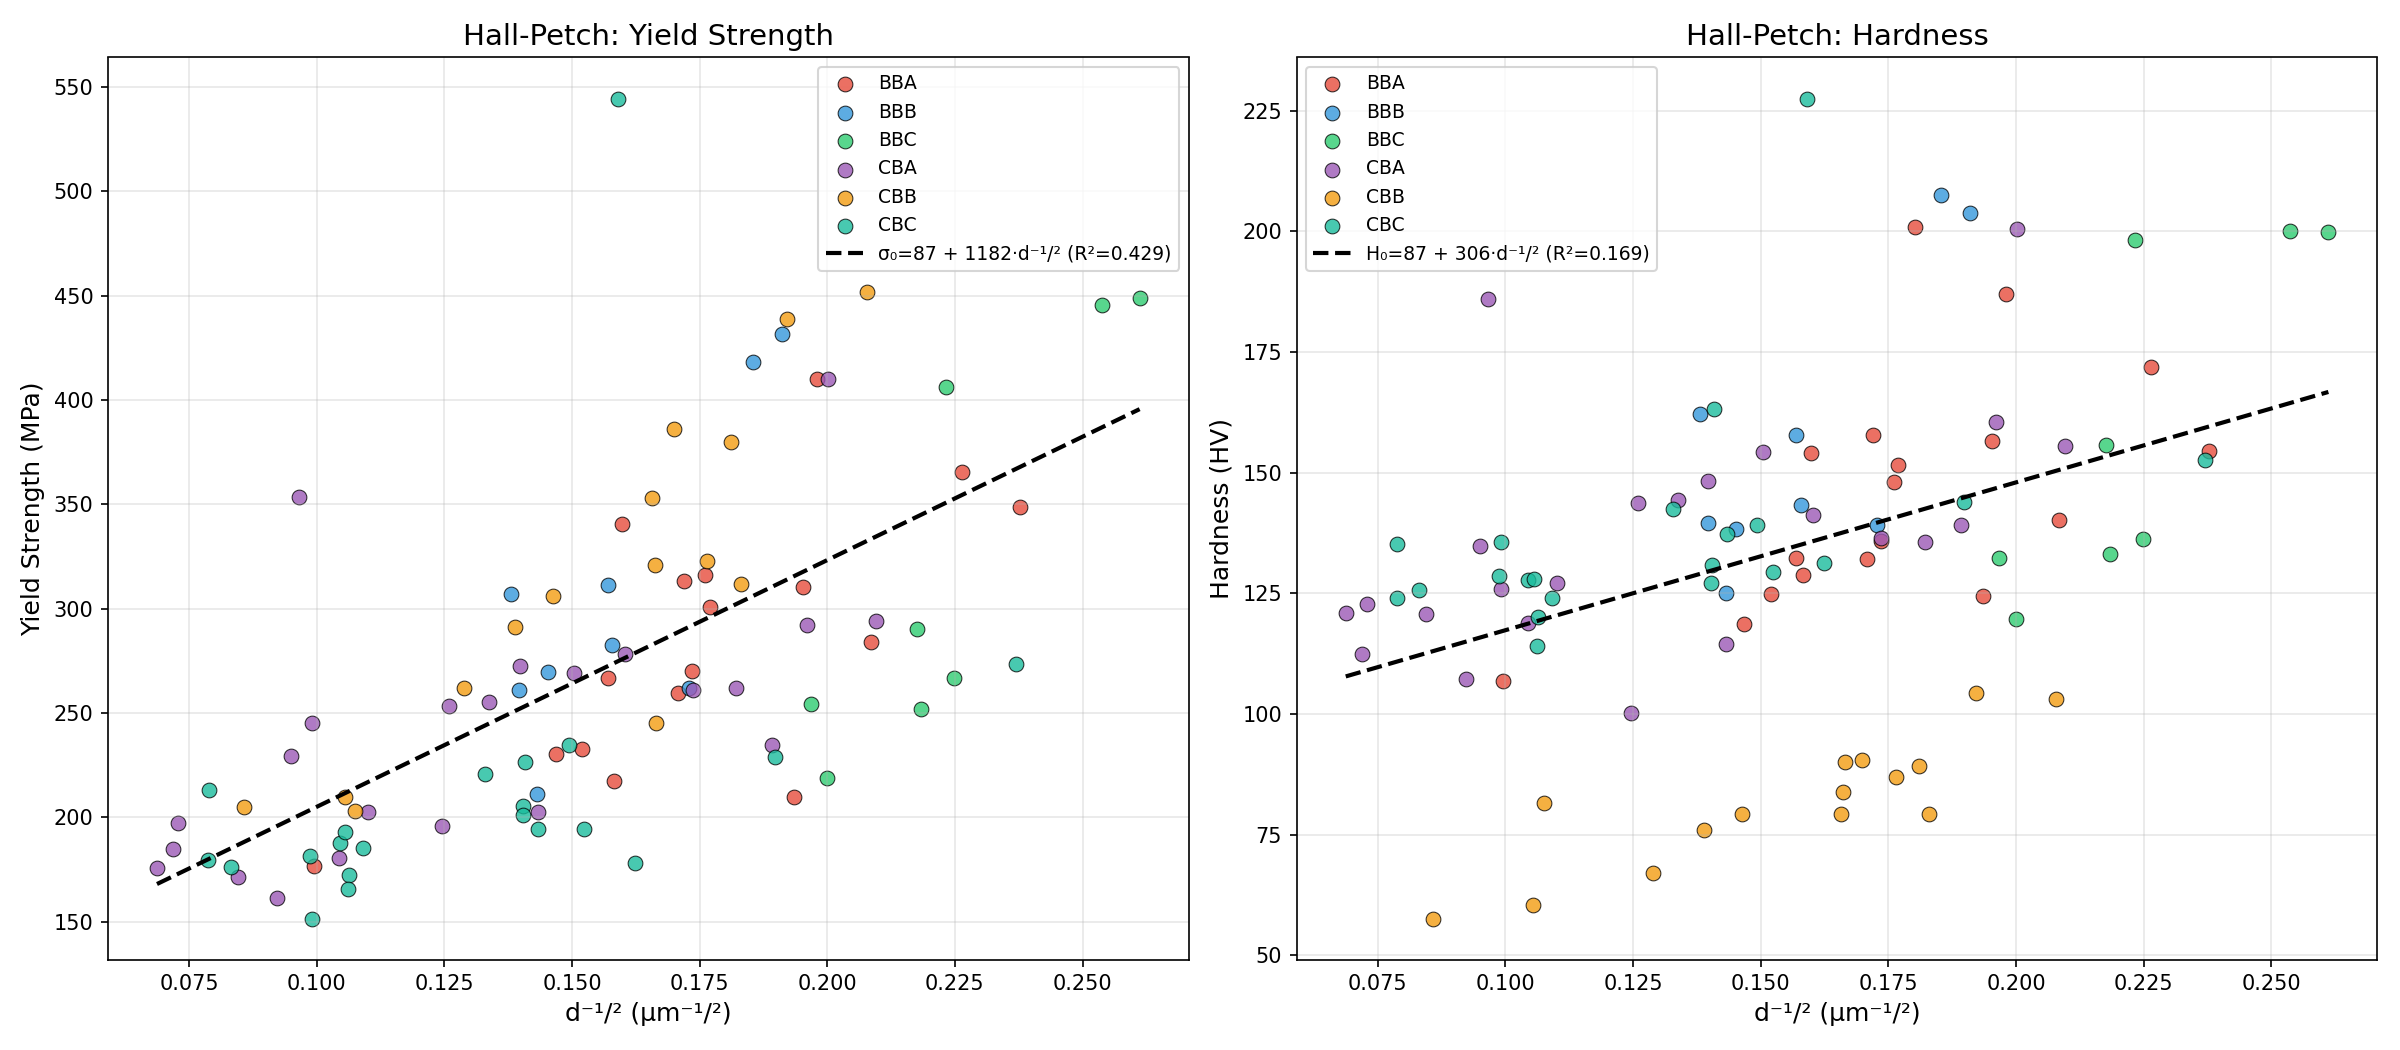
\includegraphics[width=\textwidth]{fig01_hall_petch.png}
  \caption{Classical Hall--Petch analysis: yield strength versus $d^{-1/2}$ for the 93 FCC HEAs with tensile data, colored by experimental batch. The global regression (LOO $R^2 = 0.406$) leaves substantial residual variance attributable to composition.}
  \label{fig:hall_petch}
\end{figure*}

\subsection{Tier 2 --- faithful SSS models fail quantitatively and are redundant descriptors}
\label{sec:tier2}

Implemented faithfully with Vegard's-law and rule-of-mixtures inputs, all three physics-based SSS models overpredict the friction stress of the 93-alloy panel: within a Cantor-anchored calibration (SI Section~S3), VLC overshoots the Hall--Petch-corrected experimental friction stress by 78\% (raw $R^2 = -6.92$), Toda-Caraballo by 42\% ($R^2 = -3.18$), and only calibrated Labusch lands near unit ratio (1.07, $R^2 = +0.14$); across the wider uncalibrated benchmark the overprediction spans factors of 2--28.
As standalone LOO predictors all three fall below the Hall--Petch baseline, and in a Ridge regression alongside $d^{-1/2}$ only calibrated Labusch adds value (LOO $R^2 = 0.469$ vs.\ 0.406).
The decisive test is redundancy: once the eight elemental fractions are provided as features, appending any SSS prediction changes LOO $R^2$ by less than 0.002 (composition$+$HP $= 0.654$), and the partial correlation between each SSS prediction and YS after regressing out composition is below 0.10 in magnitude for all three models.
All three formulas are deterministic functions of composition, so a flexible model with composition as input can encode any transformation they express; the physics-based encoding adds value only if it is more sample-efficient, and on this dataset it is not.

The same conclusion holds for hardness: SSS descriptors carry no independent HV signal once composition is present.
For both properties, the SSS models serve better as feature generators and physics audits than as standalone predictors---a best-practices warning quantified here by the partial-$r$ audit, which we suggest should precede any claim that a hand-built descriptor is doing physical work in an ML model.

\subsection{Tier 3 --- composition and processing: signal for YS, noise for HV}
\label{sec:tier3}

Making $\sigma_0$ composition-dependent yields the largest single gain of the ladder for yield strength (Table~\ref{tab:mmodels}, Fig.~\ref{fig:comp_hp_models}).
Adding only the V fraction (M1) raises LOO $R^2$ from 0.406 to 0.605; M3 (all seven non-Ni fractions in $\sigma_0$, constant $k_\text{HP}$) reaches LOO $R^2 = 0.652$, LOBO $R^2 = 0.625$, and external RMSE 133~\si{MPa}, and carries a PSIS-LOO stacking weight of 0.902 in the no-$\text{SD}_\text{grain}$ Bayesian comparison.
M1 and M3 are BIC-indistinguishable ($\Delta\text{BIC} = 1.4$), so the V-only model is an equally valid parsimonious choice.
The fitted $k_\text{HP} = 766$~MPa$\cdot\mu$m$^{1/2}$ sits within the FCC-HEA literature range (between CoCrFeNi at 516 and Al$_{0.3}$CoCrFeNi at 824~MPa$\cdot\mu$m$^{1/2}$; SI Section~S8), whereas the grain-only fit inflates the slope to ${\sim}1149$~MPa$\cdot\mu$m$^{1/2}$ by absorbing composition effects---V-rich alloys are systematically stronger and finer-grained ($r(V, d) = -0.24$)---so the composition-dependent intercept is what returns the slope to physically sensible values.
V dominates the friction stress ($\alpha_V = +291$~\si{MPa}, the largest positive coefficient), consistent with the Yin--Maresca--Curtin prediction that V is the optimal FCC-HEA strengthener by misfit volume~\cite{Yin2020}.
The same element plays a documented dual role at campaign level: in the risk-aware optimization that generated the B-batches, V simultaneously drove yield strength ($r = 0.84$) and $\sigma$-phase infeasibility ($r = 0.54$), with the strongest alloys and the phase failures sharing compositional points at V $= 24$~at.\%~\cite{Mulukutla2026BRAVE}---so $\alpha_V$ should be read as a within-FCC-window coefficient whose deployment envelope ends at the phase-stability boundary.
Notably, the full coefficient-versus-misfit comparison (Fig.~\ref{fig:misfit}) shows the empirical $\alpha_i$ tracking fractional volume misfit for the elements that vary appreciably across the dataset, with Al the labeled exception (largest misfit but a narrow 0--4~at.\% range).
Composition enters through $\sigma_0$, not the slope: a two-stage regression of per-alloy $k_\text{eff}$ on composition yields $R^2 = 0.006$ ($F$-test $p = 0.999$), and hierarchical Bayesian slope coefficients have uncertainties 3--4$\times$ their means.
The composition-dependent intercept mirrors the elemental-combination systematics that Yoshida et al.\ extracted from Hall--Petch fits across CoCrFeMnNi subsets~\cite{Yoshida2019acta}; the composition-independent slope, by contrast, is a statement about this dataset---single-phase solid solutions with no deliberate boundary segregants---rather than a universal rule, since boundary chemistry can nearly double $k_\text{HP}$ where segregation or nano-clustering is activated~\cite{LiKHP2024}.

Adding grain-size heterogeneity extends the hierarchy decisively.
M15 ($=$ M3 $+$ $\text{SD}_\text{grain}$ $+$ $\text{SD}_\text{grain}\cdot d^{-1/2}$) takes rank~\#1 in the $\text{SD}_\text{grain}$-augmented Bayesian comparison with stacking weight 0.89 and $\Delta\text{elpd} = 11.7$ over M3, and reaches LOO $= $ LOBO $= 0.694$---the smallest LOO$\to$LOBO gap and the highest LOBO of any closed-form YS model in this work.
Notably, $\text{SD}_\text{grain}\cdot d^{-1/2}$ is the same structural form that both symbolic-regression engines rediscover independently in Section~\ref{sec:tier5}.

For hardness the identical machinery overfits.
Every composition M-model run on HV has LOO $R^2 \leq 0.14$, and the grain-only baseline M0 is the best member of the hierarchy: composition adds variance, not signal.
The contrast with YS---where the same features lifted LOBO from 0.39 to 0.625---is the first half of the property-specific-modeling argument completed in Section~\ref{sec:contrast}.

\begin{table}[t]
\centering
\caption{Composition-dependent Hall--Petch hierarchy for YS ($\sigma_y = \sigma_0(\text{comp}) + k(\text{comp})\,d^{-1/2}$), with the $\text{SD}_\text{grain}$-augmented M15. $\Delta$BIC is relative to M3. For HV, all composition M-models have LOO $R^2 \leq 0.14$ and M0 is best.}
\label{tab:mmodels}
\small
\setlength{\tabcolsep}{4pt}
\begin{tabular}{lcccc}
\toprule
Model & Params & LOO $R^2$ & LOBO $R^2$ & $\Delta$BIC \\
\midrule
M0: baseline HP                    & 3  & 0.406 & 0.373 & 36.5 \\
M1: $\sigma_0(V)$                  & 4  & 0.605 & ---   & 1.4 \\
M3: $\sigma_0$(all 7 elem.)        & 10 & 0.652 & 0.625 & 0.0 \\
M4: $k(V)$                         & 4  & 0.598 & ---   & 3.2 \\
M6: $k$(all 7 elem.)               & 10 & 0.622 & ---   & 5.5 \\
M10: $\sigma_0$(all)$+k$(all)      & 17 & 0.650 & ---   & 17.3 \\
M11: $\sigma_0(\delta)$            & 4  & 0.456 & ---   & 31.3 \\
M15: M3$+\text{SD}_\text{grain}(\cdot d^{-1/2})$ & 12 & 0.694 & 0.694 & --- \\
\bottomrule
\end{tabular}
\end{table}

\begin{figure}[t]
  \centering
  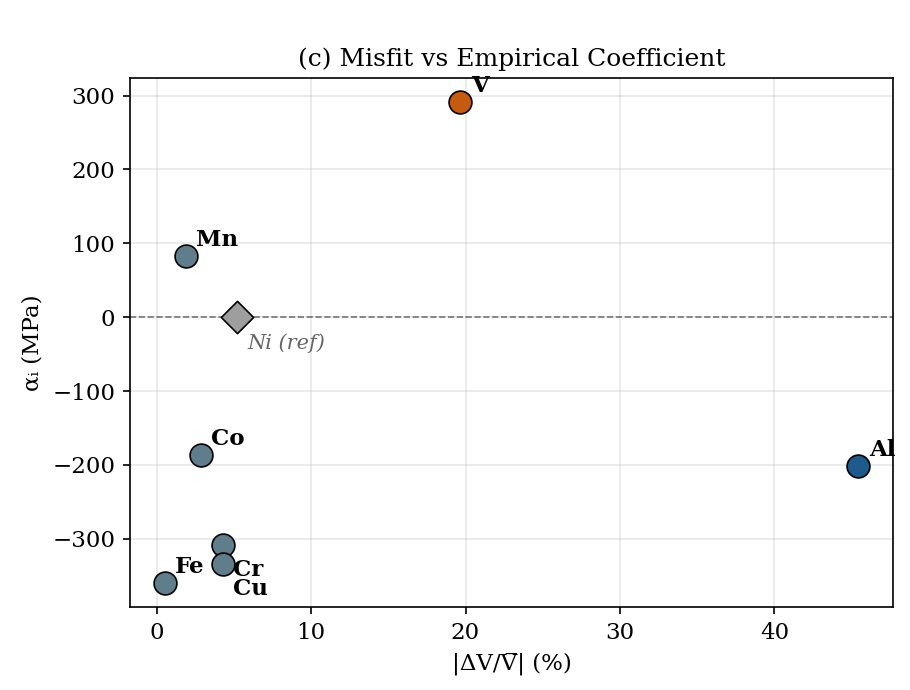
\includegraphics[width=\columnwidth]{fig_misfit_scatter.png}
  \caption{Empirical M3 friction-stress coefficients $\alpha_i$ versus fractional volume misfit $|\Delta V_i / \bar{V}|$ (Ni reference, $\alpha_\text{Ni} \equiv 0$). V's standout positive coefficient ($+291$~\si{MPa}, ${\sim}20\%$ misfit) aligns with the parameter-free Varvenne--Curtin prediction; Al has the largest misfit but a strongly negative empirical $\alpha$, reflecting its low and narrow concentration range (mean 1.1~at.\%).}
  \label{fig:misfit}
\end{figure}

\begin{figure*}[t]
  \centering
  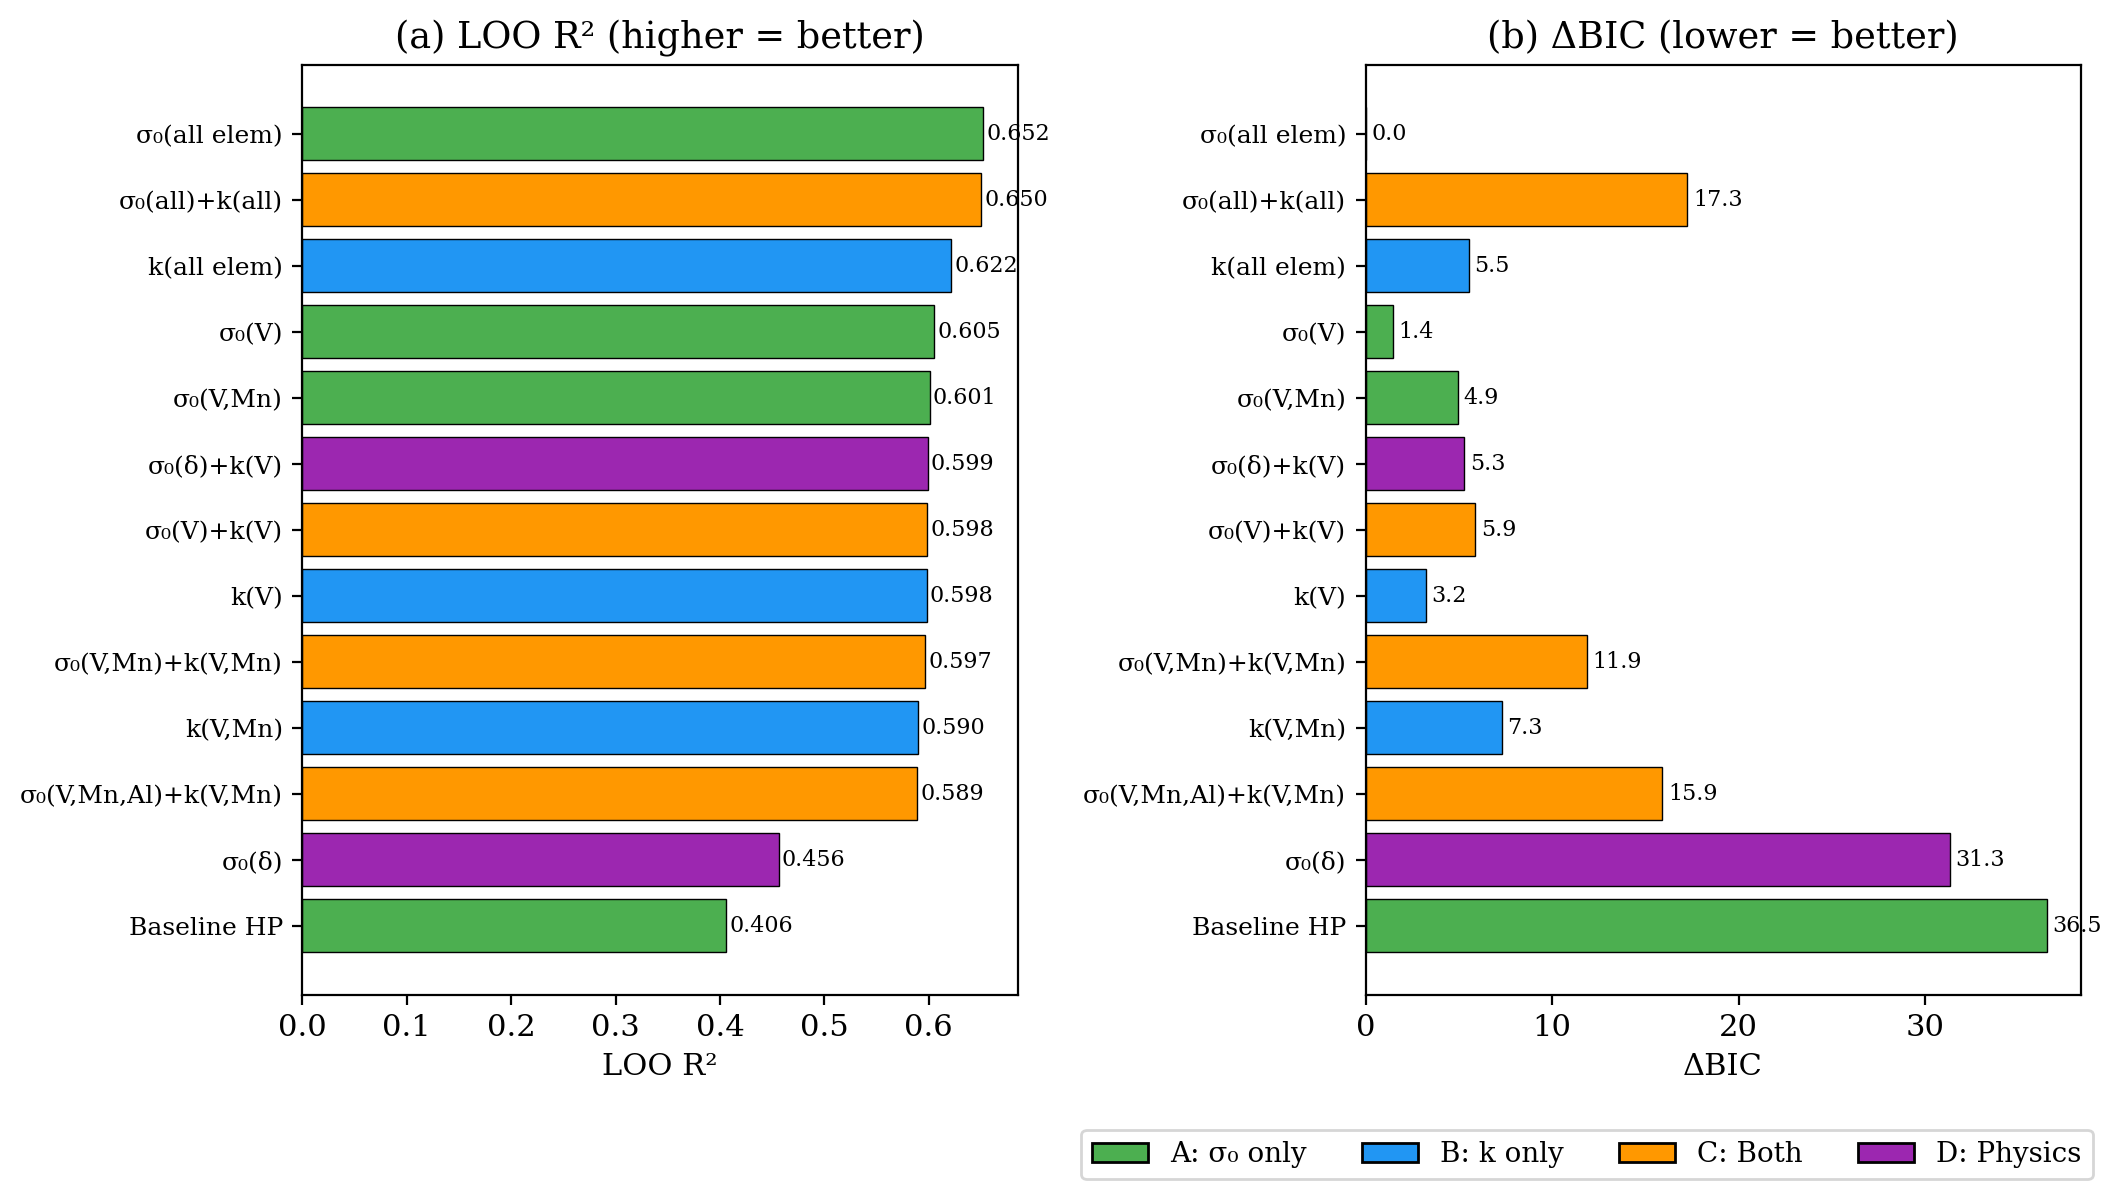
\includegraphics[width=\textwidth]{fig_comp_hp_models_ab.png}
  \caption{Composition-dependent Hall--Petch model comparison for YS across four mechanism groups (A: composition-dependent $\sigma_0$; B: composition-dependent $k$; C: both; D: physics-descriptor variants). \textbf{(a)}~LOO $R^2$ ranking. \textbf{(b)}~$\Delta$BIC relative to M3. Composition-dependent $\sigma_0$ alone tops both criteria.}
  \label{fig:comp_hp_models}
\end{figure*}

\subsection{Tier 4 --- non-linear flexibility does not pay off cross-cluster}
\label{sec:tier4}

Under the nested-CV ARMOTE panel, the best yield-strength model is linear: Bayesian ridge at the S2 tier (5-fold $R^2 = 0.69$, LOO $0.67$, LOBO $0.613$), edging the neural network (LOBO 0.57) and every tree model.
The equal-footing fair comparison sharpens the attribution (Fig.~\ref{fig:fair_heatmap}).
First, the curated Wen descriptors---not the model class---carry the YS signal: moving from grain-only (S1) to $+$Wen (S2) lifts LOBO $R^2$ from ${\approx}0.39$ to ${\approx}0.6$ for the linear and the non-linear families alike (OLS $0.394 \to 0.582$; Lasso to 0.621; LightGBM to 0.615).
Second, on equal terms linear matches or beats the trees cross-cluster: the best linear LOBO ($0.62$, Lasso at S2; ElasticNet reaches 0.617 at S4) is at or above the best non-linear LOBO (0.615, LightGBM at S2), and the gradient-boosting family peaks at 0.48.
Third, the validation failure mode is on display in the tuned panel of SI Section~S5: XGBoost with 64 engineered features posts the highest LOO $R^2 = 0.729$ of any model but collapses to LOBO $R^2 = 0.574$---an overfitting tax of 0.155 $R^2$ units that random-split CV alone would never reveal.
Dropping the rule-of-mixtures means ($\bar{\mu}$, $\delta_\mu$, $\bar{T}_m$, $\bar{a}$) from S4 barely moves the fit (ElasticNet LOBO $0.611 \to 0.617$), which strengthens the variance-over-means argument developed at Tier~5.

For hardness, nothing in either panel generalizes cross-cluster.
Within-cluster LOO scores look respectable (up to 0.48 for XGBoost at S2), but LOBO collapses to approximately zero or negative for every model at every tier (best: SVR at S1, LOBO $0.06$; adding Wen descriptors makes HV \emph{worse}, e.g.\ OLS LOBO $-0.86$ at S2).
The LOO-versus-LOBO contrast is the entire story for HV: a practitioner reading only random-split CV would deploy a hardness model that has no cross-cluster validity at all.

\begin{figure}[t]
  \centering
  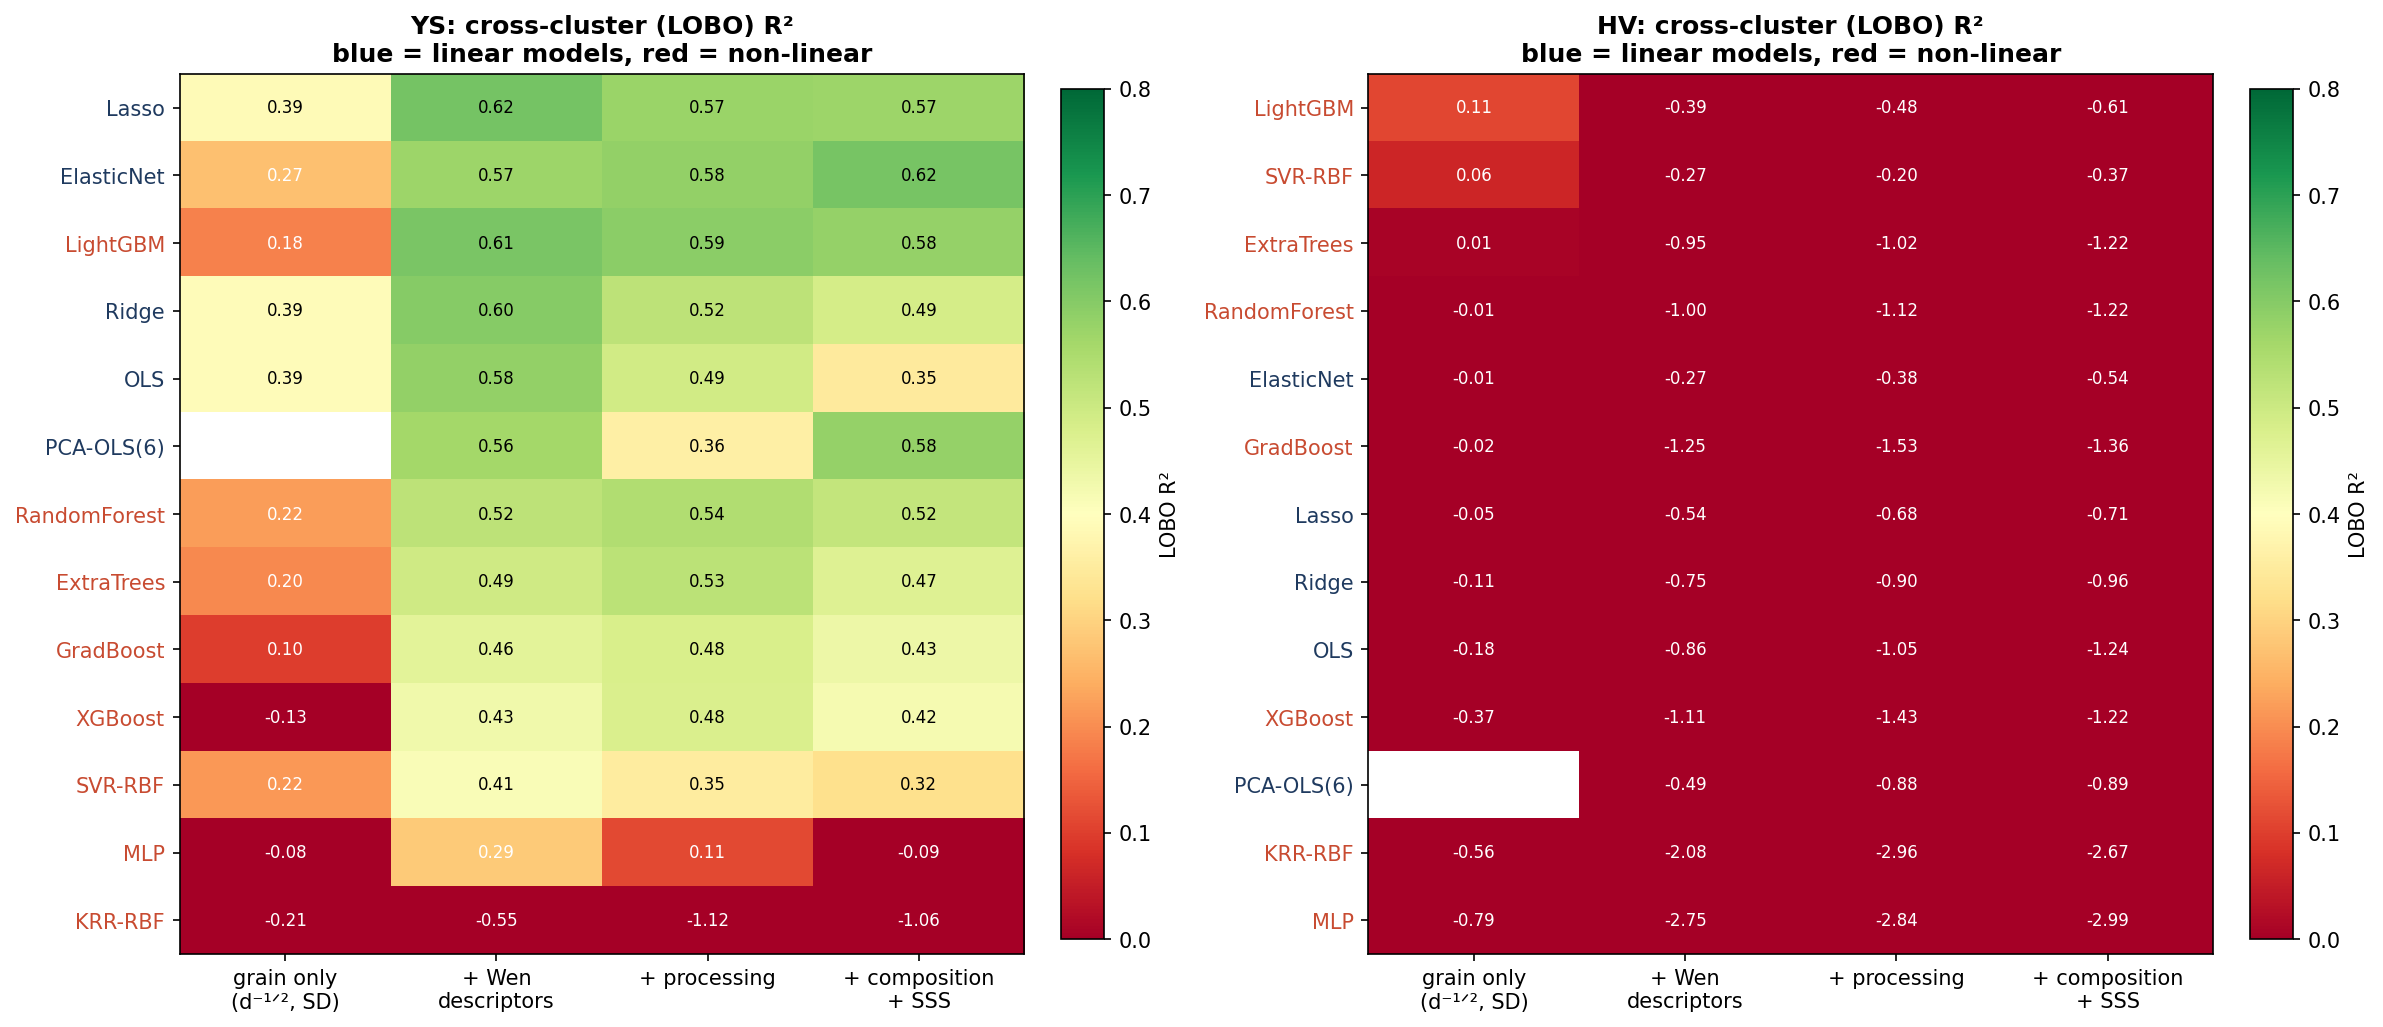
\includegraphics[width=\columnwidth]{fair_comparison_LOBO_heatmap.png}
  \caption{Equal-footing fair comparison: LOBO $R^2$ across the S1--S4 feature ladder (rows: models at zero-tuning defaults; columns: ladder tiers) for YS and HV. For YS the S1$\to$S2 (+Wen) step, not the model class, produces the lift; for HV every cell is near zero or negative beyond grain-only.}
  \label{fig:fair_heatmap}
\end{figure}

\subsection{Tier 5 --- symbolic regression: discovery, and the deployment failure mode}
\label{sec:tier5}

For yield strength, the best equations across the PySR grid come from the full ladder with unary operators (F3$+$O3).
The accuracy solution reaches LOO $R^2 = 0.765$, LOBO $R^2 = 0.668$, BIC $= 690$ (the best of any model in this work), and external RMSE 120~\si{MPa} with six fitted constants, and it is singularity-safe under the audit.
The parsimonious elbow solution, with two constants,
\begin{equation}
\label{eq:pysr_ys}
\sigma_y = \bigl(\text{SD}_\text{grain} + 1016.5\bigr)\left(d^{-1/2} + \frac{0.306}{\Omega}\right),
\end{equation}
achieves LOO $R^2 = 0.674$ and LOBO $R^2 = 0.555$.
Matched on identical curated-Wen inputs and identical scoring, PySR beats SISSO for YS (SISSO: LOO $0.485$, LOBO $0.347$ at four terms): the operator search---especially the O3 unary set---extracts more from the same inputs than SISSO's fixed feature-construction tiers.
This inverts the impression given by the unmatched comparison of SI Section~S6, where SISSO looked stronger only because it searched a richer pre-engineered Oliynyk pool.
Both engines nonetheless select the same physics: PySR places $\text{SD}_\text{grain}$ multiplicatively on the Hall--Petch term (Eq.~\ref{eq:pysr_ys}), and SISSO, once $\text{SD}_\text{grain}$ enters its pool, selects an explicit $d^{-1/2}\cdot\text{SD}_\text{grain}$ term for YS---the same form the Bayesian M15 model promotes (Section~\ref{sec:tier3}).

The deployment failure mode appears at exactly this tier.
On its original Oliynyk-style pool, SISSO discovers the four-parameter equation (SISSO Full)
\begin{equation}
\label{eq:sisso}
\sigma_y = 120.5\,\frac{\sigma_r^2}{r_\text{range}} + 9356\,\frac{d^{-1/2}}{\Delta S_\text{mix}} + 1134\,\frac{\sigma_\chi^2}{\delta_\mu} - 43.3,
\end{equation}
with LOO $R^2 = 0.665$, RMSE 46.9~\si{MPa}, LOBO $R^2 = 0.380$, and BIC 714.
The third term hides a latent singularity: Co, Fe, Mn, and Ni have shear moduli within $[75, 82]$~\si{GPa}, so ternaries from this group drive $\delta_\mu \to 0$ and predictions past 1000~\si{MPa}.
On the 82-point external set the equation fails catastrophically (RMSE 421~\si{MPa}, $R^2 = -14.8$), driven entirely by Mn-containing ternaries.
Re-running SISSO with $\delta_\mu$ excluded yields the bounded variant (SISSO Robust)
\begin{equation}
\label{eq:sisso_robust}
\sigma_y = 4806\,\frac{\sigma_r^2}{\sigma_\text{TC}} + 9187\,\frac{d^{-1/2}}{\Delta S_\text{mix}} + 6111\,(\sigma_\chi^2 - \Phi_\text{VLC}) - 110.4,
\end{equation}
which sacrifices LOO $R^2$ ($0.609$, RMSE 50.7~\si{MPa}, $\Delta_\text{LOO} = 0.056$) and a hair of LOBO ($0.358$ vs.\ $0.380$) but achieves external RMSE 163~\si{MPa} with no singularities and---uniquely among the top equations---no imputation, since it requires no $\text{SD}_\text{grain}$ measurement (Fig.~\ref{fig:external}).
Augmenting the SISSO pool with $\text{SD}_\text{grain}$ instead gives a third option: LOO $0.560$, LOBO $0.429$, external RMSE 128~\si{MPa}, singularity-safe.
The best safe PySR equation reaches external RMSE ${\approx}108$~\si{MPa}, but only by imputing $\text{SD}_\text{grain}$ on literature alloys that do not report it.

For hardness, the bounded HV elbow equation---the compact F3$+$O2 form
\begin{equation}
\label{eq:hv_elbow}
\text{HV} \approx 221.5 - 83.9\,\frac{6.93 - d}{\text{SD}_\text{grain}} + \frac{\Delta H_\text{mix}}{t_\text{hold}^2},
\end{equation}
with three fitted constants---survives refit cross-validation at LOO $R^2 = 0.727$ and LOBO $R^2 = 0.636$, making it the only HV model in this work that generalizes cross-cluster; its audited envelope excludes the near-singular regions $d \to 6.93~\si{\micro\meter}$ and $t_\text{hold} \to 0$.
Its leading term is again grain geometry: hardness rises as the grain-size distribution tightens relative to its mean.
No HV model generalizes externally under any engine: the most accurate PySR-HV and SISSO$+$SD equations contain descriptor-division singularities that blow up out-of-sample (external RMSE $10^3$--$10^4$~HV), the same failure mode as SISSO Full for YS, and even singularity-safe HV forms post strongly negative external $R^2$.
Hardness prediction beyond the training clusters remains an open problem; the honest statement of that fact is itself a product of the audit.

\begin{figure}[t]
  \centering
  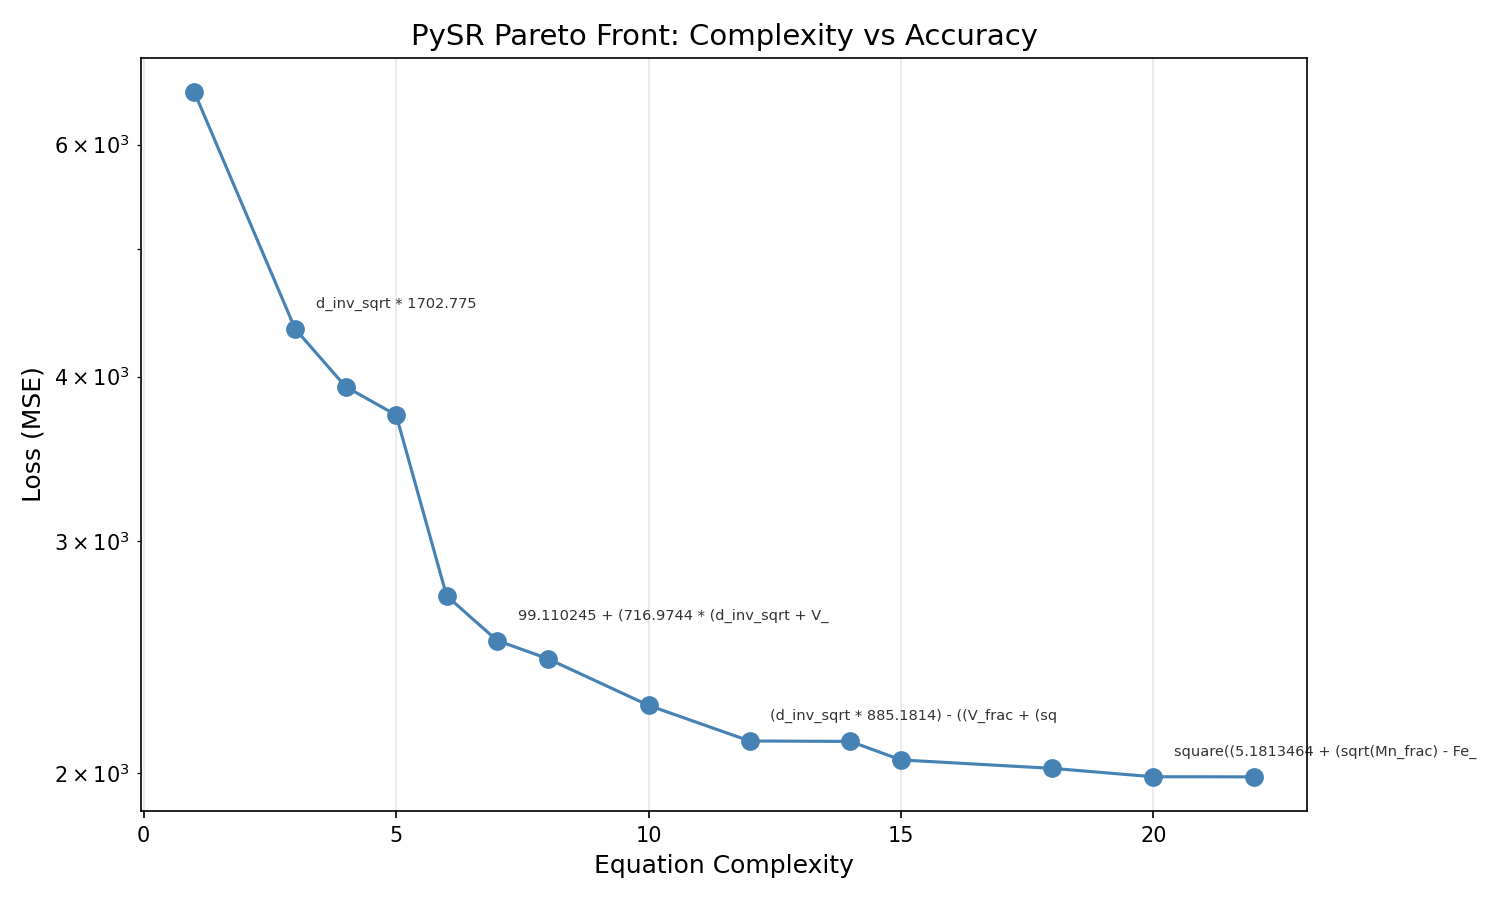
\includegraphics[width=\columnwidth]{fig08_pysr_pareto.png}
  \caption{PySR complexity--loss Pareto front for YS on the F3 (curated-Wen) $+$ O3 grid cell. The elbow (parsimonious knee, Eq.~\ref{eq:pysr_ys}) and accuracy solutions are marked; marginal gains are exhausted well before the dataset's noise ceiling.}
  \label{fig:pysr_pareto}
\end{figure}

\begin{figure*}[t]
  \centering
  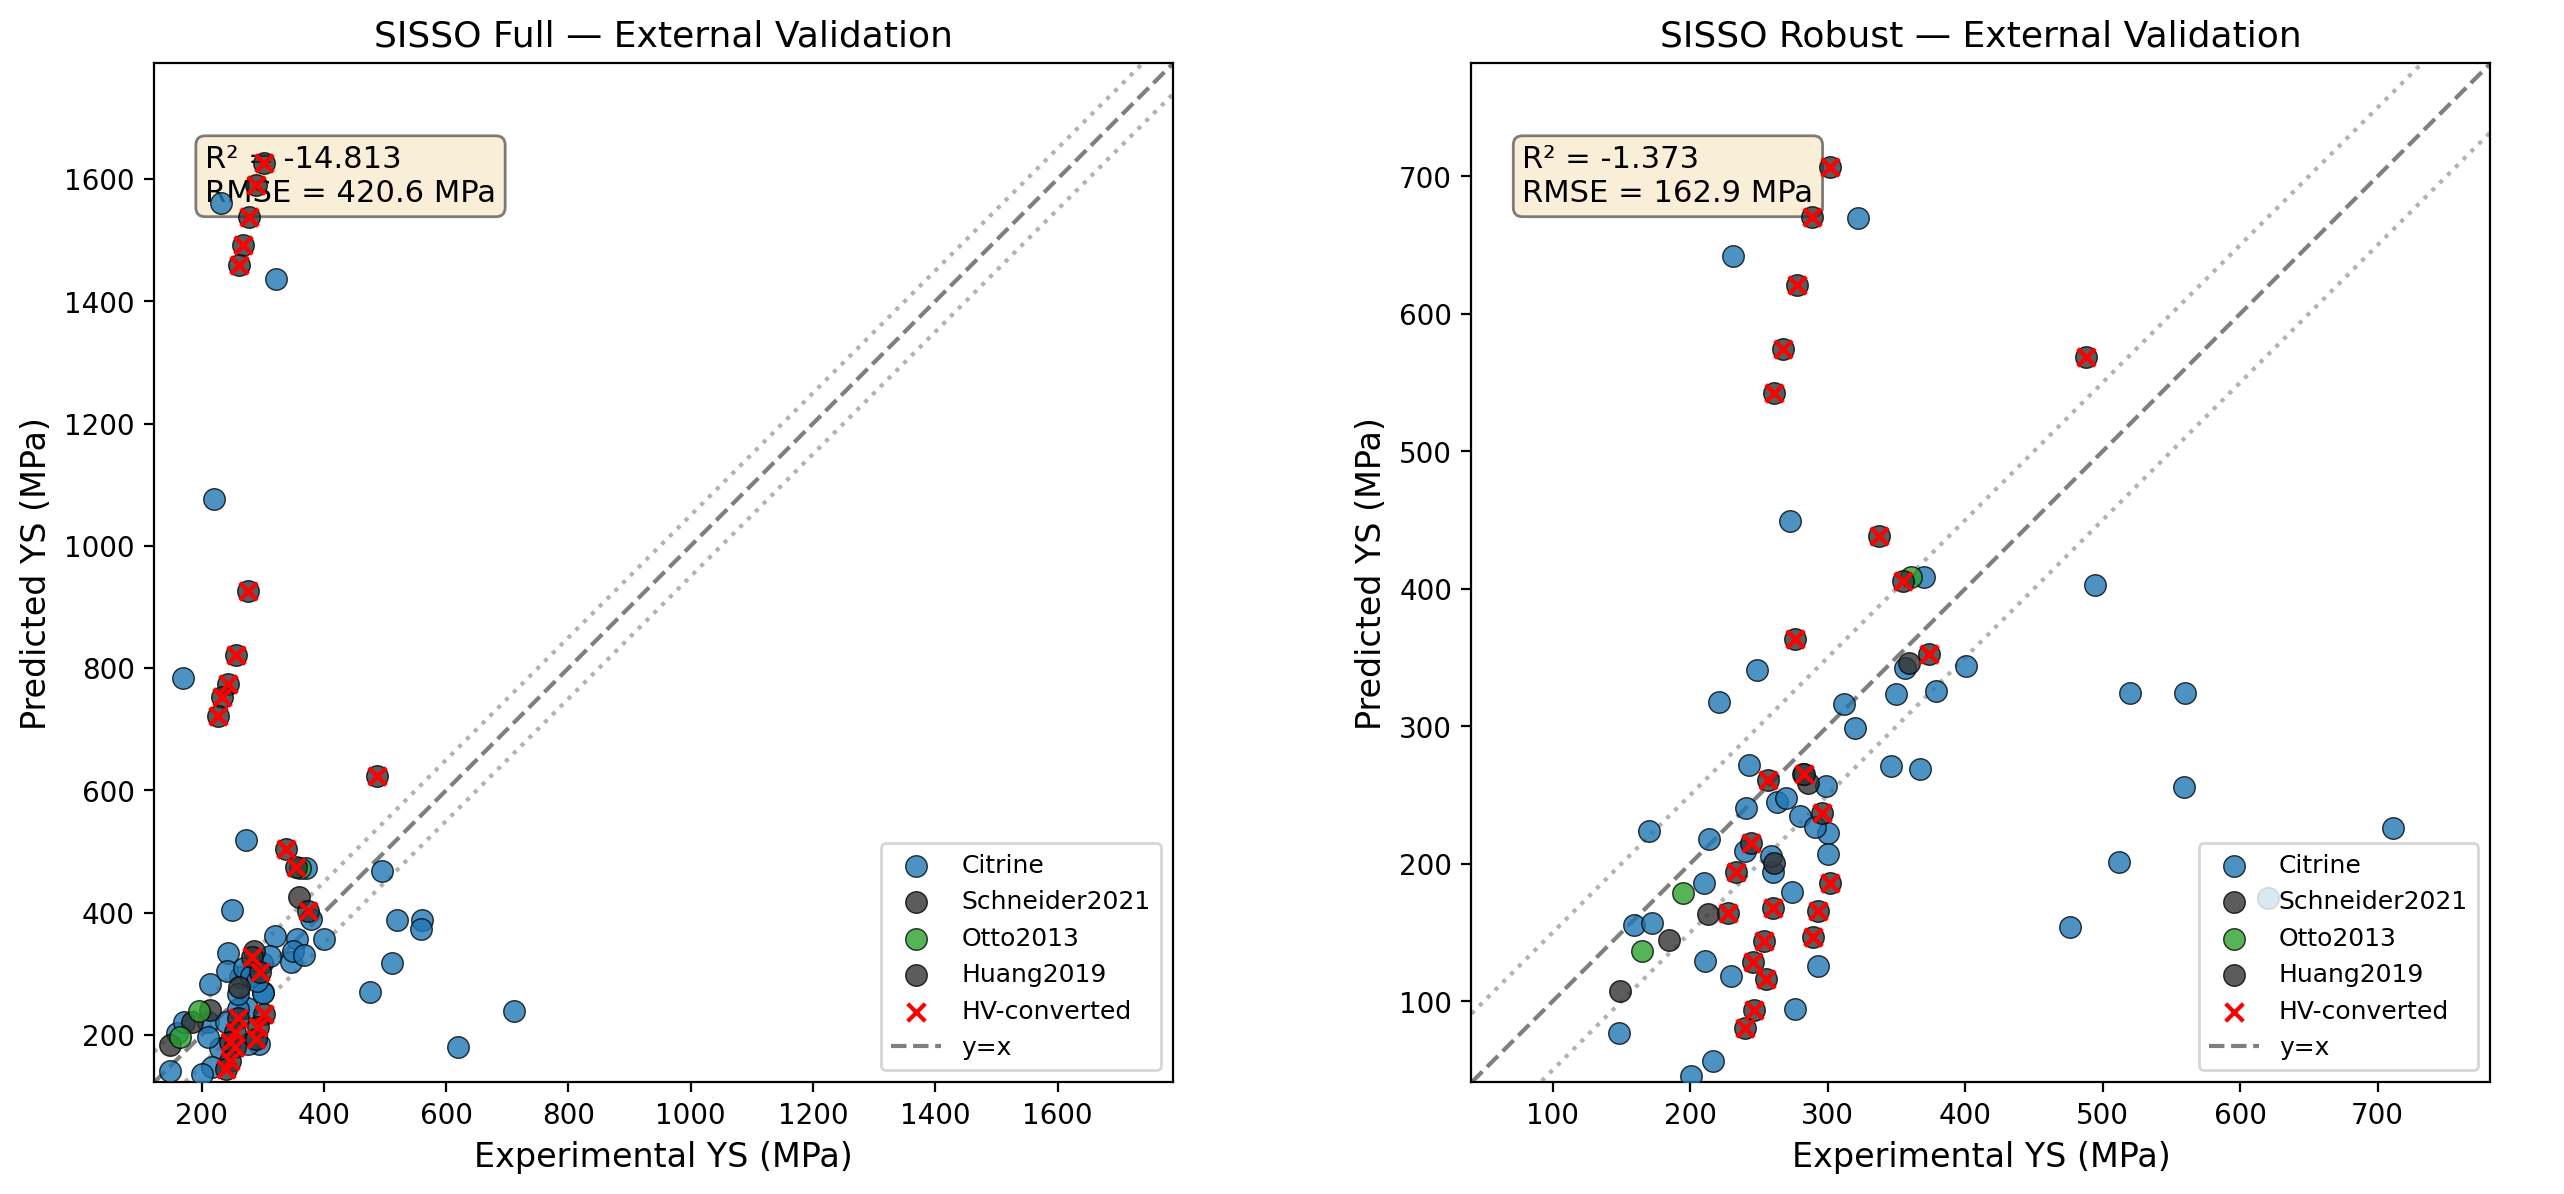
\includegraphics[width=\textwidth]{fig_external_ab.png}
  \caption{External validation on 82 independent literature points. \textbf{(Left)}~SISSO Full (Eq.~\ref{eq:sisso}): catastrophic failure ($R^2 = -14.8$, RMSE $= 421$~\si{MPa}) driven by the $\sigma_\chi^2/\delta_\mu$ singularity on Mn-containing ternaries. \textbf{(Right)}~SISSO Robust (Eq.~\ref{eq:sisso_robust}): the pathology disappears (RMSE $= 163$~\si{MPa}, bias $-32$~\si{MPa}). M3 (not shown) yields RMSE $= 133$~\si{MPa}.}
  \label{fig:external}
\end{figure*}

\subsection{Three engines converge on grain-size heterogeneity}
\label{sec:convergence}

The single most consequential physical finding is structural, not numerical: three independent search mechanisms---PySR's genetic programming, SISSO's sparse operator screening, and the Bayesian M-model hierarchy---each arrive at a $\text{SD}_\text{grain}\cdot d^{-1/2}$ coupling, for both properties where applicable.
PySR multiplies the Hall--Petch term by $(\text{SD}_\text{grain} + \text{const})$ (Eq.~\ref{eq:pysr_ys}); SISSO selects $d^{-1/2}\cdot\text{SD}_\text{grain}$ explicitly for both YS and HV once the feature is available; and M15 wins the Bayesian comparison by adding exactly this interaction (LOO $=$ LOBO $= 0.694$).
Because the three engines share no search mechanism, their agreement is evidence that grain-size heterogeneity---not just the mean grain size---governs strengthening in these alloys: real polycrystals carry a distribution of grain sizes, the finest grains yield last and carry disproportionate load, and a single-$d$ Hall--Petch law cannot express that.
Convergent evidence of this kind is our proposed criterion for reading an ML-discovered term as physics rather than curve-fitting.

The discovered term has a substantial theoretical pedigree, although---to our knowledge---no prior study has used the measured grain-size standard deviation as an explicit predictor.
Classical dispersion micromechanics established decades ago that yield stress depends on the width of the grain-size distribution, not only its mean: volume-weighted Hall--Petch averaging~\cite{Kurzydlowski1990}, self-consistent models over lognormal distributions in which the distribution's standard deviation enters the yield stress explicitly~\cite{Berbenni2007}, and experimental work on welded steels showing that mean-$d$ Hall--Petch fits mispredict strength when the distribution broadens~\cite{Lehto2014}.
That literature predicts \emph{softening} as the distribution widens at fixed mean; the heterostructure literature predicts the opposite, with engineered wide or bimodal grain-size distributions generating hetero-deformation-induced (HDI) back-stress strengthening above rule-of-mixtures expectations~\cite{Wang2002,ZhuWu2019}.
Our fitted signs place the two properties on opposite sides of this competition: the PySR yield-strength equation (Eq.~\ref{eq:pysr_ys}) strengthens with $\text{SD}_\text{grain}$, HDI-like, while the hardness elbow (Eq.~\ref{eq:hv_elbow}) softens as the distribution widens at fixed $d$, as classical dispersion theory predicts---a contrast consistent with the property-specific-modeling thesis of Section~\ref{sec:contrast}.

An independent linear check points the same way.
PCA-OLS on the curated-Wen$+$$\text{SD}_\text{grain}$ set (six components, 88\% of variance) is stable if unspectacular (5-fold $0.525$, LOO $0.516$, LOBO $0.441$), and its reconstructed importances rank $\Delta H_\text{mix}$, $d^{-1/2}$, $\Delta\chi$, and $\Omega$ at the top---the same features PySR's compact YS equations select.
Two unrelated methods agreeing on the governing variables indicates those variables are a property of the data, not of any one method.

\subsection{Hardness--strength correspondence and its limits}
\label{sec:tabor}

The effective Tabor factor across the dataset is $C_\text{eff} = \text{HV(MPa)}/\sigma_y = 5.13 \pm 1.36$, well above the classical 3 (Fig.~\ref{fig:tabor}); within the generalized Tabor framework this measures a flow-stress ratio $\sigma_f(0.08)/\sigma_y = 1.71$ and an early-strain hardening exponent $n_\text{eff} = \ln(C_\text{eff}/3)/\ln 40 \approx 0.15 \pm 0.07$, consistent with the strong work hardening of FCC HEAs sampled over the early post-yield regime.
The elevated ratio agrees with HEA-wide compilations, which find that HV/3 tracks the \emph{ultimate} rather than the yield strength in work-hardenable FCC HEAs~\cite{Tian2021,Fan2021}: the constraint factor itself is not anomalous; the excess sits in the hardening between yield and the representative indentation strain.
The per-alloy spread implies that no single conversion factor reliably transforms HV to $\sigma_y$ across alloys ($\pm 25\%$ at fixed HV).

Used as a ranking proxy, HV shows a Simpson's paradox: the global Spearman correlation between HV and YS ranks is $\rho = 0.46$ while per-batch correlations span 0.70--0.95.
The campaigns isolate the cause: pooling the fixed-processing B-campaign preserves the ranking ($\rho = 0.95$), pooling the processing-swept C-campaign destroys it ($\rho = 0.09$), yet conditioning on grain size does not recover coherence (partial $\rho(\text{HV},\text{YS}\,|\,d) = 0.24$).
Composition---V especially---is the primary scrambler, with grain size acting as a confounder through its shared Hall--Petch correlation with both properties; the empirical fit $\log C_\text{eff} = 1.36 + 0.10\,\log d - 2.06\,x_V$ quantifies both effects.
HV therefore ranks alloys reliably only within a narrow composition window; cross-campaign screening should measure $\sigma_y$ directly or apply a V-content correction.
Full rank-correlation analysis is given in SI Section~S7.

\begin{figure*}[t]
  \centering
  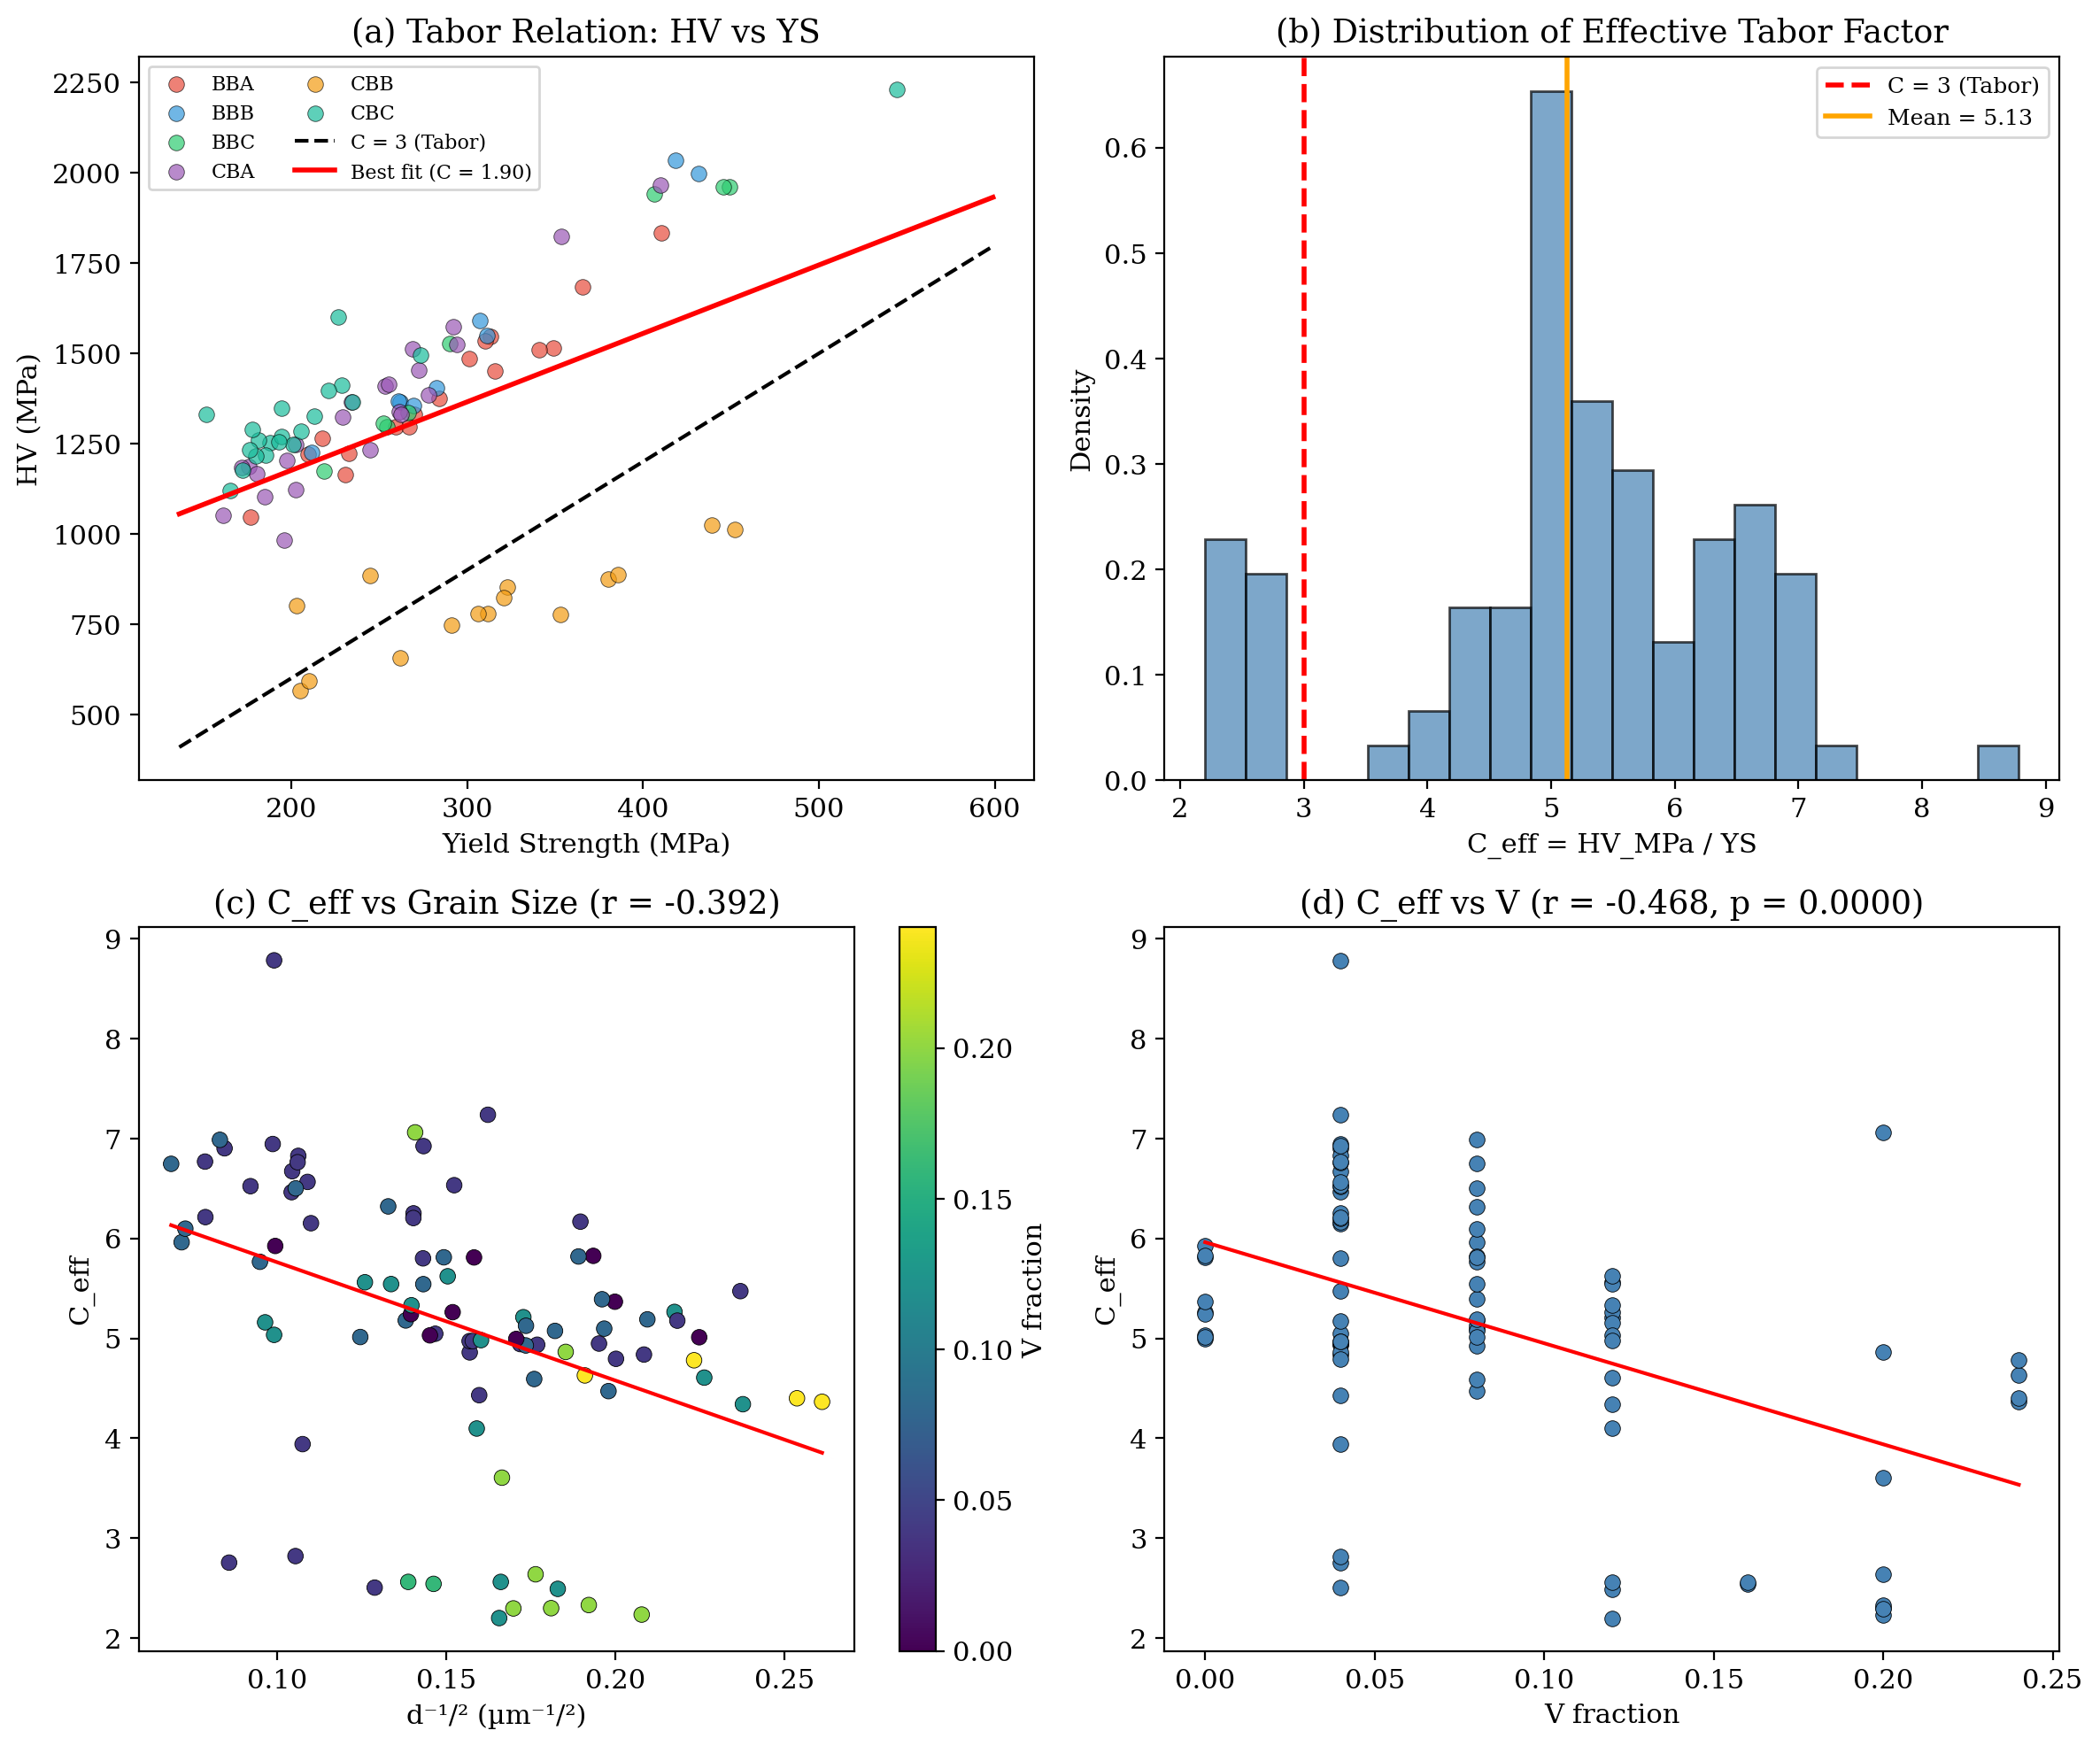
\includegraphics[width=\textwidth]{fig09_tabor_relation.png}
  \caption{Hardness--yield strength correspondence. (a)~HV versus $\sigma_y$ by batch against the classical Tabor line. (b)~Distribution of $C_\text{eff} = \text{HV(MPa)}/\sigma_y$ (mean 5.13 vs.\ classical 3). (c)~$C_\text{eff}$ versus $d^{-1/2}$ ($r = -0.39$). (d)~$C_\text{eff}$ versus V fraction ($r = -0.47$).}
  \label{fig:tabor}
\end{figure*}

\subsection{Deployment-aware model selection}
\label{sec:verdict}

No single model wins every criterion, and the winner changes with the deployment constraint (Table~\ref{tab:verdict}).
For peak YS accuracy the PySR accuracy equation leads (LOO 0.765, LOBO 0.668); for the highest cross-cluster closed form with $\text{SD}_\text{grain}$ available, M15 (LOO $=$ LOBO $= 0.694$); for deployment without grain-size-distribution measurements, M3 (external RMSE 133~\si{MPa}, no imputation) or SISSO Robust (163~\si{MPa}, bounded, descriptor-only).
For hardness the bounded $\text{SD}_\text{grain}$ elbow (Eq.~\ref{eq:hv_elbow}) is the only cross-cluster survivor, composition models are not recommended at all, and no model is externally reliable.
Reporting this table---rather than a single leaderboard number---is itself one of the framework's guardrails.

\begin{table*}[t]
\centering
\caption{Best-model verdict by deployment criterion. Every cross-validated entry reports both LOO and LOBO; external RMSE in MPa (YS). ``Imputation'' flags models requiring $\text{SD}_\text{grain}$ values that independent literature does not report.}
\label{tab:verdict}
\small
\setlength{\tabcolsep}{5pt}
\begin{tabular}{@{}llp{8.6cm}@{}}
\toprule
Property & Criterion & Recommended model \\
\midrule
YS & Peak accuracy & PySR accuracy eq.\ (LOO 0.765, LOBO 0.668, BIC 690, ext.\ 120) \\
YS & Highest cross-cluster closed form ($\text{SD}_\text{grain}$ available) & M15 Bayesian composition-HP $+$ $\text{SD}_\text{grain}\cdot d^{-1/2}$ (LOO $=$ LOBO $=$ 0.694) \\
YS & Deployable interpretable, no imputation & M3 composition-HP (LOO 0.652, LOBO 0.625, ext.\ 133, stacking weight 0.902) \\
YS & Parsimony $+$ interpretability & SISSO Full (4 params, BIC 714) --- but $\delta_\mu$ singularity; deploy the Robust variant \\
YS & Honest cross-cluster linear ML & Lasso/ElasticNet on the fair ladder (LOBO 0.62) / Bayesian ridge, ARMOTE S2 (LOBO 0.613) \\
YS & Deployment without $\text{SD}_\text{grain}$ or composition fractions & SISSO Robust (ext.\ 163, LOBO 0.358, singularity-safe, no imputation) \\
YS & Best external error ($\text{SD}_\text{grain}$ available/imputed) & PySR (${\approx}108$) / SISSO$+$SD (128) / M3 (133, no imputation) \\
\midrule
HV & Best deployable in-sample & $\text{SD}_\text{grain}$ Hall--Petch elbow, Eq.~\ref{eq:hv_elbow} (LOO 0.73, LOBO 0.64, 3 params) \\
HV & Linear/composition models & Not recommended --- all M-models LOO $\leq$ 0.14 (composition overfits HV) \\
HV & External generalization & None reliable --- division terms create singularities (ext.\ RMSE $10^3$--$10^4$) \\
HV & Mechanistic reading & Grain-geometry-dominated; Tabor $C_\text{eff} = 5.13$ \\
\bottomrule
\end{tabular}
\end{table*}

\subsection{Property-specific modeling is essential --- the YS versus HV contrast}
\label{sec:contrast}

Carrying both properties through the identical ladder yields the capstone contrast of Table~\ref{tab:contrast}: the same features, the same validation, and the same model families give opposite answers for YS and HV.
Composition is signal for YS (it shifts $\sigma_0$; M3 LOBO 0.625) and noise for HV (all M-models LOO $\leq 0.14$); YS models generalize cross-cluster (LOBO 0.61--0.69) while for HV only the grain-based equation survives (0.64) and everything else is at or below zero; YS deploys externally at 108--163~\si{MPa} RMSE while no HV model deploys at all.
A universal strength--hardness model would necessarily mislead for at least one property, and the Tabor analysis shows the two are linked by a composition- and grain-size-dependent factor, not a constant.
That the same protocol exposes this contrast---rather than papering over it with a pooled score---is the practical payoff of property-specific modeling under honest validation.

\begin{table*}[t]
\centering
\caption{Identical methodology, opposite conclusions: the YS versus HV contrast.}
\label{tab:contrast}
\small
\setlength{\tabcolsep}{5pt}
\begin{tabular}{@{}lll@{}}
\toprule
Axis & Yield strength & Vickers hardness \\
\midrule
Governing physics & composition ($\sigma_0$) $+$ Hall--Petch backbone & grain geometry ($\text{SD}_\text{grain}\cdot d^{-1/2}$) \\
Composition effect & shifts $\sigma_0$ --- helps (M3 LOBO 0.625) & overfits (all M-models LOO $\leq$ 0.14) \\
Best model & PySR equation / M15 / M3 Hall--Petch & $\text{SD}_\text{grain}$ Hall--Petch elbow (Eq.~\ref{eq:hv_elbow}) \\
Cross-cluster (LOBO) & generalizes (0.61--0.69) & only grain-based survives (0.64); rest $\leq 0$ \\
External / deployment & M3 133, SISSO Robust 163~\si{MPa} (no imputation) & no model generalizes externally \\
Strength--hardness link & --- & Tabor $C_\text{eff} = \text{HV}/\sigma_y = 5.13$ (HV $\neq 3\sigma_y$) \\
\bottomrule
\end{tabular}
\end{table*}

% ============================================================
% 5. DISCUSSION
% ============================================================
\section{Discussion}
\label{sec:discussion}

\subsection{Which method suits which property, and why}
\label{sec:family_reading}

Each model family earns a specific role rather than a rank.
Classical Hall--Petch is the indispensable floor: it anchors the physics, calibrates expectations (LOO 0.41 for YS, 0.14 for HV), and exposes---through its batch-to-batch parameter variation---the need for composition terms and cluster-out validation.
The linear M-models are the interpretability workhorses for YS: M3 gives a mechanistically transparent $\sigma_0(\text{comp}) + k_\text{HP}\,d^{-1/2}$ partition whose coefficients can be checked against theory (V's dominance matches parameter-free Varvenne--Curtin predictions~\cite{Yin2020}), and it deploys externally without imputation.
Physics-descriptor hierarchies serve as audits: the SSS models fail as predictors but their failure is informative, locating the error in Vegard's-law inputs rather than the theoretical framework---VLC with DFT-derived misfit volumes achieves quantitative accuracy for equimolar alloys~\cite{Varvenne2016,Moitzi2022}, and with experimentally measured lattice misfits and elastic constants it rationalizes the hardness variation across 24 single-phase FCC Co-Cr-Fe-Mn-Ni alloys~\cite{Bracq2019}---and the partial-$r$ redundancy test disciplines what a descriptor is allowed to claim.
Non-linear ML is the stress test: if a tree ensemble with every feature and a tuning budget cannot beat a linear model cross-cluster, the relationship in the deployable regime is effectively linear in the right features, and the trees' LOO edge is measurement of batch memorization rather than physics.
Symbolic regression is the discovery engine and the sharpest deployment risk at once: it produced both the best YS model in this work and the most catastrophic external failure, in the same family, distinguishable only by the audit.

The property determines the winner because the underlying physics differs.
Yield strength is a yield-point property with an additive friction-stress structure that composition shifts smoothly, so linear-in-composition models and compact symbolic forms both work.
Vickers hardness convolves yield with early-strain work hardening ($C_\text{eff} = 3\,\sigma_f(0.08)/\sigma_y$), and work-hardening capacity in these alloys is governed by grain geometry more than by chemistry---hence the grain-geometry dominance, the failure of composition models, and the collapse of cross-cluster generalization for every HV model except the $\text{SD}_\text{grain}$ form.

\subsection{Four failure modes, four guardrails}
\label{sec:guardrails}

The framework's central claim is that each measured failure mode has an inexpensive guardrail.
The physics failure (SSS overprediction by 2--28$\times$) is guarded by using ML as auditor: benchmark the physics model on the dataset before trusting it as a feature, and prefer variance-type descriptors over rule-of-mixtures means, which are inert across concentrated alloys that share similar averages by design ($\sigma_r^2$ varies 30-fold across our panel while $\bar{W}$ varies by $\pm 12\%$).
The descriptor failure (redundancy once composition is present, partial $r < 0.10$) is guarded by the partial-correlation audit, run before any claim that a hand-built descriptor does independent work.
The validation failure (LOO flatters; XGBoost $0.729 \to 0.574$; every HV model collapsing under LOBO) is guarded by reporting 5-fold, LOO, and LOBO together and headlining the LOO$\to$LOBO gap---materials datasets are almost always clustered by campaign, family, or synthesis route; cluster-out validation is the honest deployment test~\cite{Meredig2018}; and dataset redundancy compounds the optimism, since near-duplicate compositions leak between random folds~\cite{LiMDHIT2024}, exactly the pseudo-replication our 23\% shared-composition fraction produces under LOO.
The deployment failure (SISSO Full's hidden $\delta_\mu$ pole; the PySR-HV division singularities) is guarded by the singularity audit on independent data and by preferring bounded functional forms; the cost of the guardrail is small ($\Delta$LOO $= 0.056$ for SISSO Robust) against a five-fold external-error reduction.

\subsection{$\sigma_0$ versus $k_\text{HP}$, and what the interaction features mean}
\label{sec:sigma0_khp}

Tree-model importance analyses (SI Section~S5) rank composition$\times$grain-size interaction features highly, which could be misread as a composition-dependent Hall--Petch slope.
The direct tests say otherwise: per-alloy $k_\text{eff}$ regression on composition gives $R^2 = 0.006$, and M3 with a single global slope matches the flexible alternatives.
The interactions act as proxies for the composition-dependent $\sigma_0$, not as evidence that $k_\text{HP}$ varies.
Physical mechanisms for composition-dependent slopes exist---solute segregation modifying boundary cohesion and slip transmission~\cite{Cordero2016,He2014}, demonstrated dramatically by the Mo-segregation-driven $k_\text{HP} = 1100$~MPa$\cdot\mu$m$^{1/2}$ of Ref.~\cite{LiKHP2024}---but at $n = 93$, with single-phase chemistries selected against segregation and with the present design's confounding between composition and processing (SI Section~S8), any such effect sits below the detection threshold.
The genuine grain-size refinement of this work lies elsewhere: in the second moment of the grain-size distribution.
$\text{SD}_\text{grain}\cdot d^{-1/2}$ is selected by three independent engines, survives cluster-out validation (M15, LOO $=$ LOBO $= 0.694$), and carries a physical reading---load partitioning across a grain-size distribution---that classical single-$d$ Hall--Petch cannot express.
Notably, this is the constructive face of the same SR machinery whose destructive face is the singularity: handled with the audit, the engines discover physics; without it, they manufacture pathology.

\subsection{A transferable protocol, not an FCC-HEA result}
\label{sec:protocol}

Although demonstrated on FCC HEAs, nothing in the protocol is specific to them, and Table~\ref{tab:protocol} states what transfers and why.
What is FCC-HEA-specific: the coefficients (e.g., $k_\text{HP} = 766$~MPa$\cdot\mu$m$^{1/2}$, $\alpha_V = +291$~\si{MPa}, $C_\text{eff} = 5.13$), the V-dominated $\sigma_0$ signal, and the particular winning equations.
What is general: the feature-ladder logic (every structural-property problem has a physics backbone plus optional descriptors), the redundancy audit (any descriptor derived from composition can be encoded by a flexible model given composition), the variance-over-means principle (means wash out in concentrated or heterogeneous systems), cluster-out validation (materials data are clustered wherever they come from campaigns or families), the singularity audit (any deployed analytical model in any field), and multi-engine convergence as the criterion for reading a discovered term as mechanism.
The preference for compact interpretable forms over black-box models in deployment also has direct empirical support beyond this study: in systematic benchmarks on materials datasets, interpretable models trail black-box regressors only marginally when interpolating and match or beat them in a substantial fraction of extrapolation tasks~\cite{Muckley2023}---and extrapolation is exactly the regime alloy design occupies.
Readers working in BCC HEAs, conventional multicomponent alloys, ceramics, or composites can lift the workflow directly: each new system re-runs the staircase rather than starting over.

\begin{table*}[t]
\centering
\caption{The transferable best-practices protocol: each guardrail, the failure mode it prevents (as measured in this work), and why it transfers beyond FCC HEAs.}
\label{tab:protocol}
\small
\setlength{\tabcolsep}{5pt}
\begin{tabularx}{\textwidth}{@{}>{\raggedright\arraybackslash}p{4.4cm}>{\raggedright\arraybackslash}p{4.8cm}>{\raggedright\arraybackslash}X@{}}
\toprule
Best practice & Guards against & Why it transfers \\
\midrule
Build a feature ladder from the physics backbone up, scoring each tier & Reading a rich-model win as physics when it is feature engineering & Every structural-property problem has a known backbone $+$ optional descriptors; the ladder isolates marginal value \\
Audit descriptor redundancy (partial correlation) before trusting a descriptor & Crediting hand-built descriptors that composition already encodes (here partial $r < 0.10$) & Holds wherever descriptors are derived from composition (ceramics, conventional alloys, MOFs) \\
Prefer variance/heterogeneity descriptors over rule-of-mixtures means & Means washing out the signal ($\bar{\mu}$, $\bar{T}_m$, $\bar{a}$ inert; $\text{SD}_\text{grain}$ decisive) & General to concentrated solid solutions and microstructurally heterogeneous materials \\
Report 5-fold $+$ LOO $+$ cluster-out (LOBO) $+$ external; headline the LOO$\to$LOBO gap & Random-split CV overselling models that fail on new regions (XGBoost $0.729 \to 0.574$) & Materials datasets are almost always clustered by campaign, family, or route \\
Singularity/deployment audit of every closed form on independent data & In-sample-beautiful equations that diverge in deployment (ext.\ RMSE 421~\si{MPa}) & Any deployed analytical model in any field; bounded variants are the fix \\
Trust a mechanism only when independent engines converge on it & Mistaking a single-method fit for physics & If unrelated search strategies rediscover the same form ($\text{SD}_\text{grain}\cdot d^{-1/2}$), the effect is real \\
\bottomrule
\end{tabularx}
\end{table*}

\subsection{Limitations}
\label{sec:limitations}

The 94 alloys come from two BO campaigns at a single group with shared synthesis and characterization protocols, so generalization to other processing classes (severe plastic deformation, additive manufacturing) is untested, and the composition space is unevenly sampled (Al restricted to 0--4~at.\%, Ni-rich throughout).
BO-driven sampling means the alloys concentrate near campaign-specific Pareto fronts rather than covering the simplex~\cite{Mulukutla2026BRAVE}, and LOBO folds differ in difficulty (hull coverage 0.29--0.87 across held-out batches); per-batch LOBO breakdowns are given in SI Section~S8.
Although M15 and the SR equations promote $\text{SD}_\text{grain}$, the term's external validation is limited because independent literature rarely reports grain-size distributions---which is itself a reporting recommendation of this work.
Monte Carlo and bootstrap diagnostics bound the parameter sensitivities (e.g., $k_\text{HP}$ shifts $\pm 39\%$ under grain-size measurement perturbation, M3 composition coefficients under $\pm 15\%$); the within-replicate design does not support a clean test of $k_\text{HP}(\text{comp})$ at fixed processing.
The 23\% of alloys sharing exact compositions constitutes the dataset-redundancy problem known to inflate random-split metrics~\cite{LiMDHIT2024}; LOBO is our structural control for it, since shared compositions never straddle a batch boundary's train/test split within a campaign iteration.
Finally, hyperparameter tuning in the legacy 17-model panel used the full dataset before LOO, an optimism we quantified and then eliminated in the nested ARMOTE-CV and zero-tuning fair-comparison panels.

% ============================================================
% 6. CONCLUSIONS
% ============================================================
\section{Conclusions}
\label{sec:conclusions}

Machine-learning property prediction in sparse, clustered materials data is not unsafe by nature; it is unsafe by default.
This work turned that observation into a working protocol and demonstrated it end-to-end on the yield strength and Vickers hardness of 94 FCC HEAs: build a physics-anchored feature ladder, audit descriptor redundancy before trusting hand-built physics, prefer variance and heterogeneity descriptors over rule-of-mixtures means, validate with LOO and cluster-out LOBO together and headline the gap, audit every closed form for singularities on independent data, and accept a discovered term as mechanism only when independent engines converge on it.

The demonstrated payoff runs in both directions.
Constructively, the protocol delivered the strongest models in every deployment regime: for YS a symbolic-regression equation with LOO $R^2 = 0.765$ and LOBO $R^2 = 0.668$, the Bayesian composition-Hall--Petch models M3 (deployable without imputation, external RMSE 133~\si{MPa}) and M15 (LOO $=$ LOBO $= 0.694$), and the discovery---confirmed independently by PySR, SISSO, and the Bayesian hierarchy---that grain-size heterogeneity enters through $\text{SD}_\text{grain}\cdot d^{-1/2}$.
As auditor, the same machinery measured the four failure modes it guards against: solid-solution models overpredicting 2--28$\times$ and going redundant at partial $r < 0.10$; leave-one-out flattering a tree ensemble by 0.155 $R^2$ units relative to cluster-out truth; a best-BIC equation hiding a singularity that quintuples its external error; and every composition-based hardness model overfitting outright, with HV shown to be grain-geometry-dominated and externally unpredictable by any current model.

The coefficients belong to this alloy system; the workflow does not.
Extensions we consider warranted: applying the identical ladder and validation protocol to BCC HEAs, conventional multicomponent alloys, ceramics, and composites; replacing Vegard's-law misfits with first-principles volumes; microstructure-aware descriptors beyond the first two moments of the grain-size distribution; routine reporting of grain-size distributions (not just means) in experimental strength studies; and LOBO-validated transfer learning across processing routes and alloy families.
Each new system re-runs the staircase rather than starting over; that is the contribution we intend to be reused.

% ============================================================
% BACK MATTER
% ============================================================
\section*{CRediT authorship contribution statement}

[TODO(submission): per-author CRediT roles.]

\section*{Declaration of competing interest}

The authors declare that they have no known competing financial
interests or personal relationships that could have appeared to
influence the work reported in this paper.

\section*{Acknowledgments}

The research was sponsored by the Army Research Laboratory and was
accomplished under Cooperative Agreement Number W911NF-22-2-0106. The
views and conclusions contained in this document are those of the
authors and do not represent the official
policies, either expressed or implied, of the Army Research Laboratory
or the US Government. The US Government is authorized to reproduce and
distribute reprints for Government Purposes, notwithstanding any
copyright notation herein.

We acknowledge Dr.\ Anup and his group at Texas A\&M
University for the use of their XRD Bruker D8 Discover instrument, Texas A\&M's Materials Characterization Facility for the use
of their EBSD-capable FIB-SEM, and Texas
A\&M's High Performance Research Computing group for computational infrastructure.

\section*{Data and code availability}

All analysis code, derived data, and figure-generation scripts are
available in the companion repository [TODO(submission): repository URL].
An archival snapshot is deposited on Zenodo:
\url{https://doi.org/10.5281/zenodo.XXXXXXX} [TODO(submission): mint record].
The raw experimental dataset and the 82-point external-validation set are included in the repository.

% ============================================================
% REFERENCES
% ============================================================
\bibliographystyle{elsarticle-num}
\bibliography{references}

\end{document}
